%\documentclass[journal]{vgtc}                % final (journal style)
\documentclass[review]{vgtc}		          % review (journal style)
%\documentclass[widereview]{vgtc}             % wide-spaced review
%\documentclass[preprint,journal]{vgtc}       % preprint (journal style)
%\documentclass[electronic,journal]{vgtc}     % electronic version, journal

%% Uncomment one of the lines above depending on where your paper is
%% in the conference process. ``review'' and ``widereview'' are for review
%% submission, ``preprint'' is for pre-publication, and the final version
%% doesn't use a specific qualifier. Further, ``electronic'' includes
%% hyperreferences for more convenient online viewing.

%% Please use one of the ``review'' options in combination with the
%% assigned online id (see below) ONLY if your paper uses a double blind
%% review process. Some conferences, like IEEE Vis and InfoVis, have NOT
%% in the past.

%% Please note that the use of figures other than the optional teaser is not permitted on the first page
%% of the journal version.  Figures should begin on the second page and be
%% in CMYK or Grey scale format, otherwise, colour shifting may occur
%% during the printing process.  Papers submitted with figures other than the optional teaser on the
%% first page will be refused.

%% These three lines bring in essential packages: ``mathptmx'' for Type 1
%% typefaces, ``graphicx'' for inclusion of EPS figures. and ``times''
%% for proper handling of the times font family.

\usepackage{mathptmx}
\usepackage{graphicx}
\usepackage{times}

%%%%%%%%%%%%%%%%%%%%%%%%%%%%
%% Add-by-Abon 08/21/13
%%%%%%%%%%%%%%%%%%%%%%%%%%%%
\newcommand{\remove}[1]{}

%%%%%%%%%%%%%%%%%%%%%%%%%%%%
%% Add-by-Abon 09/14
%%%%%%%%%%%%%%%%%%%%%%%%%%%%
%\usepackage[font=scriptsize]{caption}
\usepackage{amsthm}
\usepackage{amsmath}
%\usepackage{subfigure}
\usepackage{subfig}
\usepackage{subfloat}
\usepackage{wrapfig}


\newenvironment{packed_enumerate}{
\begin{enumerate}
  \setlength{\itemsep}{1pt}
  \setlength{\parskip}{0pt}
  \setlength{\parsep}{0pt}}{\end{enumerate}
}

\newenvironment{packed_itemize}{
\begin{itemize}
  \setlength{\itemsep}{1pt}
  \setlength{\parskip}{0pt}
  \setlength{\parsep}{0pt}}{\end{itemize}
}

\newcommand{\specialcell}[2][c]{%
  \begin{tabular}[#1]{@{}c@{}}#2\end{tabular}}
%%%%%%%%%%%%%%%%%%%%%%%%%%%%
%% Add-by-Abon 09/14
%%%%%%%%%%%%%%%%%%%%%%%%%%%%

%% We encourage the use of mathptmx for consistent usage of times font
%% throughout the proceedings. However, if you encounter conflicts
%% with other math-related packages, you may want to disable it.

%% This turns references into clickable hyperlinks.
\usepackage[bookmarks,backref=true,linkcolor=black]{hyperref} %,colorlinks
\hypersetup{
  pdfauthor = {},
  pdftitle = {},
  pdfsubject = {},
  pdfkeywords = {},
  colorlinks=true,
  linkcolor= black,
  citecolor= black,
  pageanchor=true,
  urlcolor = black,
  plainpages = false,
  linktocpage
}

% Change the colon in figure and table caption to dot. e.g. Change Fig. 2: to Fig. 2.
\captionsetup{labelsep=period}


% Use Sans Serif font for the caption.
\captionsetup{font={sf,small}}
% Do not align the caption to the middle even if the caption has only 1 line.

\captionsetup{singlelinecheck=off}

%% If you are submitting a paper to a conference for review with a double
%% blind reviewing process, please replace the value ``0'' below with your
%% OnlineID. Otherwise, you may safely leave it at ``0''.
\onlineid{102}

%% declare the category of your paper, only shown in review mode
\vgtccategory{Research}

%% allow for this line if you want the electronic option to work properly
\vgtcinsertpkg

%% In preprint mode you may define your own headline.
%\preprinttext{To appear in an IEEE VGTC sponsored conference.}

%% Paper title.

\title{Efficient Range Distribution Query for Visualizing Scientific Data}

%% This is how authors are specified in the journal style

%% indicate IEEE Member or Student Member in form indicated below
\author{Roy G. Biv, Ed Grimley, \textit{Member, IEEE}, and Martha Stewart}
\authorfooter{
%% insert punctuation at end of each item
\item
 Roy G. Biv is with Starbucks Research, e-mail: roy.g.biv@aol.com.
\item
 Ed Grimley is with Grimley Widgets, Inc., e-mail: ed.grimley@aol.com.
\item
 Martha Stewart is with Martha Stewart Enterprises at Microsoft
 Research, e-mail: martha.stewart@marthastewart.com.
}

%other entries to be set up for journal
\shortauthortitle{Biv \MakeLowercase{\textit{et al.}}: Global Illumination for Fun and Profit}
%\shortauthortitle{Firstauthor \MakeLowercase{\textit{et al.}}: Paper Title}

%% Abstract section.
\abstract{
Visualization applications implicitly run queries on the data to retrieve distributions and statistical measures derivable from distributions. Distribution based data summaries can substitute for the raw data to answer statistical queries of different kinds. However, frequent access to the raw data is no longer practical, if possible at all, for answering large number of queries on large-scale data. Our work addresses the issue by accelerating \emph{range distribution query}, which returns the distribution of an axis-aligned query region. Maintaining the interactivity of such query results is a challenging task because the workload, which affects the response time, of such queries scales up with the data and the query size. In this paper, we present framework for answering range distribution queries for any arbitrary region in constant time, regardless of data and query size. We adapt an integral histogram based data structure to bound the workload which is a combination of computation, I/O and communication cost. We propose two novel transformations of this data structure -- a decomposition and a similarity-driven indexing -- to reduce the huge storage cost associated with it. In addition to studying performance of query, we also demonstrate the benefits that our technique offers to  visualization applications which directly or indirectly require distributions.
} % end of abstract

%% Keywords that describe your work. Will show as 'Index Terms' in journal
%% please capitalize first letter and insert punctuation after last keyword
%\keywords{Distributions, Indexing, Query, Large data.}

%% ACM Computing Classification System (CCS). 
%% See <http://www.acm.org/class/1998/> for details.
%% The ``\CCScat'' command takes four arguments.

%\CCScatlist{ % not used in journal version
% \CCScat{K.6.1}{Management of Computing and Information Systems}%
%{Project and People Management}{Life Cycle};
% \CCScat{K.7.m}{The Computing Profession}{Miscellaneous}{Ethics}
%}

%% Uncomment below to include a teaser figure.
%\teaser{
%\centering
%\includegraphics[width=16cm]{CypressView}
%\caption{In the Clouds: Vancouver from Cypress Mountain.}
%}

%% Uncomment below to disable the manuscript note
%\renewcommand{\manuscriptnotetxt}{}

%% Copyright space is enabled by default as required by guidelines.
%% It is disabled by the 'review' option or via the following command:
% \nocopyrightspace

%%%%%%%%%%%%%%%%%%%%%%%%%%%%%%%%%%%%%%%%%%%%%%%%%%%%%%%%%%%%%%%%
%%%%%%%%%%%%%%%%%%%%%% START OF THE PAPER %%%%%%%%%%%%%%%%%%%%%%
%%%%%%%%%%%%%%%%%%%%%%%%%%%%%%%%%%%%%%%%%%%%%%%%%%%%%%%%%%%%%%%%%

\begin{document}

%% The ``\maketitle'' command must be the first command after the
%% ``\begin{document}'' command. It prepares and prints the title block.

%% the only exception to this rule is the \firstsection command
%\firstsection{Introduction}

\maketitle

\section{Introduction}
\label{sec:intro}
%%

Query-driven techniques have become increasingly popular for exploring and visualizing scientific datasets. Statistical summaries such as mean, standard deviation, entropy and higher order moments computed from distributions of spatial sub-ranges are useful for feature extraction, uncertainty quantification, multi-resolution analysis, and data reduction, just to name a few. Useful local statistics are often derived from distributions commonly represented as histograms. In general, this type of queries is known as \emph{range distribution query}~\cite{martin13}, which returns the distribution of an axis-aligned query region of any arbitrary size. Traditionally, such queries are supported by running a sequential scan through the raw data. However, as the data size grows, frequently accessing large subsets of the raw data increases workload, which leads to slower query response time. This is because both the time and space complexity of such queries are proportional to the number of data points in the query region.

The importance of range distribution query is apparent from its wide use, directly or indirectly, in a number of visualization algorithms~\cite{Hixel11, uncertain3d11, qdv11} (explained in more detail in Section~\ref{sec:relwork}). Since the approach of scanning raw data does not scale well with data size, it is important to devise strategies to maintain the interactivity of a distribution query engine. In this paper, we propose to transform the raw data into a data structure which stores and uses pre-computed distributions to answer distribution query for any range in constant time. However, we need to address two major challenges to make this approach effective:
%%
\begin{packed_itemize}
%%
\item {\bf Query workload:} The workload of the query engine should be low and constant regardless of the query size and data size. The workload refers to a combination of the cost of accessing data in memory, the I/O cost associated with reading files from the disk, if needed, and also the communication cost of exchanging partial query results, if needed.
%%
\item {\bf Distribution storage:} The number of pre-computed distributions required to answer range distributions queries is as large as the number of data points. We must minimize the storage cost of the pre-computed distributions so that the query can be run on commodity desktops with moderate amount of storage. 
%%
\end{packed_itemize}

To bound the query workload, we adapt a data structure called integral distribution~\cite{integhist05}. It is an extension of the summed area table (SAT) proposed by Crow~\cite{SAT84} which, at each location of the data, stores the sum of the attribute values from the origin up to that location. SAT can compute the sum of an attribute in any rectangular region in constant time, regardless of the region size. Similarly, integral distribution can compute the distribution of any query region by accessing pre-computed distributions only at the corner points of the query region. Hence, the workload is bounded by the number of corner points which is same for any query of any size. 

The benefit, however, comes at the cost of huge storage cost. The total space required to store an integral histogram is in the order of $O(N*K)$ for $N$ data points and $K$ number of bins per histograms. This is prohibitively large even for data sets of moderate size. We address this storage issue by proposing a set of transformations to stored integral distributions to make them compression-friendly. After the proposed transformations - a decomposition followed by an indexing - are run on the integral distributions, any off-the-shelf compression technique can be employed to achieve much higher space saving. We propose the following transformations for integral distributions: First, we decompose them into a hierarchy of block distributions pertaining to power-of-two length sub-ranges. We propose a novel similarity-based indexing technique to be employed on these block distributions. These transformations lead to significant space saving and much faster query performance.

The rest of the paper is organized as follows. Section~\ref{sec:relwork} summarized the related work on management and storage of distribution data. The following Section~\ref{sec:distqueryframework} describes our framework including the transformations proposed to integral distribution, similarity-based indexing of distributions and the query mechanism. Section~\ref{sec:application} demonstrates how our technique benefits visualization applications. A detailed quantitative study of the framework is presented in Section~\ref{sec:analysis},  followed by discussion (Section~\ref{sec:discussion}) and conclusion (Section~\ref{sec:conclusion}). 

\section{Related Work}
\label{sec:relwork}
%%
\paragraph{Distribution-based Techniques:} The use of distributions in data analysis and visualization is ever-growing.  Scientific simulations often produce outcomes with uncertainty, making a distribution-based approach the most suitable for post-processing~\cite{Hixel11}. Sometimes the data itself come in the form of distributions. For example, multi-run simulations generate ensemble data which produce distribution of the outcomes from individual runs. To analyze data of this type, various algorithms that use distribution queries have been developed.  Examples include fuzzy isosurface computation from uncertain data~\cite{Hixel11}, and analysis of uncertain vector fields~\cite{uncertain3d11}. Even for conventional data, Johnson and Huang have proposed a distribution-based query to identify regions having a certain type of distribution~\cite{johnson09}. Similarly, Gosink et al. have shown that distributions of sub-regions of varying sizes are useful for feature extraction and segmentation~\cite{qdv11}. Block level distributions have also been used in spatio-temporal data analysis~\cite{transgraph11}. ProbVis~\cite{probvis12} is another distribution query engine. However, all these methods access the raw data to compute and display distributions whereas we aim at answering queries without having to access the raw data. Hence, our method can extend any of these query-driven techniques to large data when raw data access is not recommended.

Distributions of scalar values and their attributes play a critical role in designing transfer function for volume rendering~\cite{semiautomatic98, localhistogram06} and predicting isosurface statistics~\cite{carrhist06}. Distributions are also critical in information theory based visualization since local and global distributions are needed to compute a suite of information theoretic metrics~\cite{Xu10}.

\paragraph{Efficient Storage of Distributions:} Exact query processing on large databases became infeasible especially for certain applications such as online analytical processing (OLAP), giving way to fast and approximate query return based on pre-computed distributions~\cite{Buccafurri02}. In another approach, histograms have been treated as
signals and various basis transforms such as wavelet~\cite{WaveletHist98} and SVD~\cite{SVD97} have been used to compress them. In visualization community, a recent work has proposed a statistical method of approximating histograms by Gaussian Mixture kernels to reduce the storage overhead~\cite{GMM12}. Another recent work has converted local distributions to sparse representations to reduce the overhead of computing probabilistic mipmaps from gigapixel images~\cite{Hadwiger12}. Efficient storage and retrieval of histograms is studied in other areas such as computer vision~\cite{CHOG2012} as well. 
%Visualization~\cite{Kao02, Luo03} of pointwise histograms is usually performed using the data. 

\paragraph{Similarity-based Methods:} The presence of self-similarity in various types of data has been  used for feature detection, encoding and other purposes. Shechtman and Irani~\cite{selfsimilarity07} have utilized self-similarity within an image and across multiple sequences in a video frame to detect visual entities. Jacquin~\cite{Jacquin92}, 
%based on the theoretical insight provided by Barnsley et al.~\cite{Barnsley88}, 
introduced a self-similarity based coding technique, known as fractal coding, for images. In fractal coding, the image to be encoded is partitioned into spatial blocks called \emph{range blocks} ($R_k$). Another smaller set of partitions, called \emph{domain blocks}, of the same image is created to serve as representative templates. The range block set is mapped to the domain block set in such a way that the range blocks, and hence the data can be reconstructed only from a set of iterative functions. 

In this paper, we observe the great extent of similarity present across distributions coming from the same data. and develop a similarity-base matching framework for representing histograms in scientific data sets. 





\section{Proposed Framework}
\label{sec:distqueryframework}
%%
%%
In this paper, we present a framework to rapidly return the distribution of any arbitrarily large axis-aligned spatial region in a volumetric data. When such queries are answered using the raw data, the response time is a function of the size and shape of the query region, which is manageable for relatively smaller data which fits in memory. However, in most real applications, the data is too big for memory and hence, is partitioned and stored in the disk as multiple blocks. In this case, not only the query region is too big for a sequential scan, it spans across multiple data blocks, requiring numerous files to be loaded to answer it. As a result, the time required to scan the data as well as the I/O cost associated with loading these data blocks add to the query workload. Figure~\ref{fig:ih_mainbenefit} (left) schematically presents the problem. Moreover, if the data blocks are loaded in different processors in a distributed memory system, communication is needed among processors to aggregate the locally computed partial distributions. This communication cost also adds to the workload which is reflected in the response time.
%%%%%%%%%%%%%%%%%%%
%% Diagram begins
%%%%%%%%%%%%%%%%%%%
\begin{figure}[tb]
\centering
	%\subfloat[]{\label{fig:loadfilterscan}
	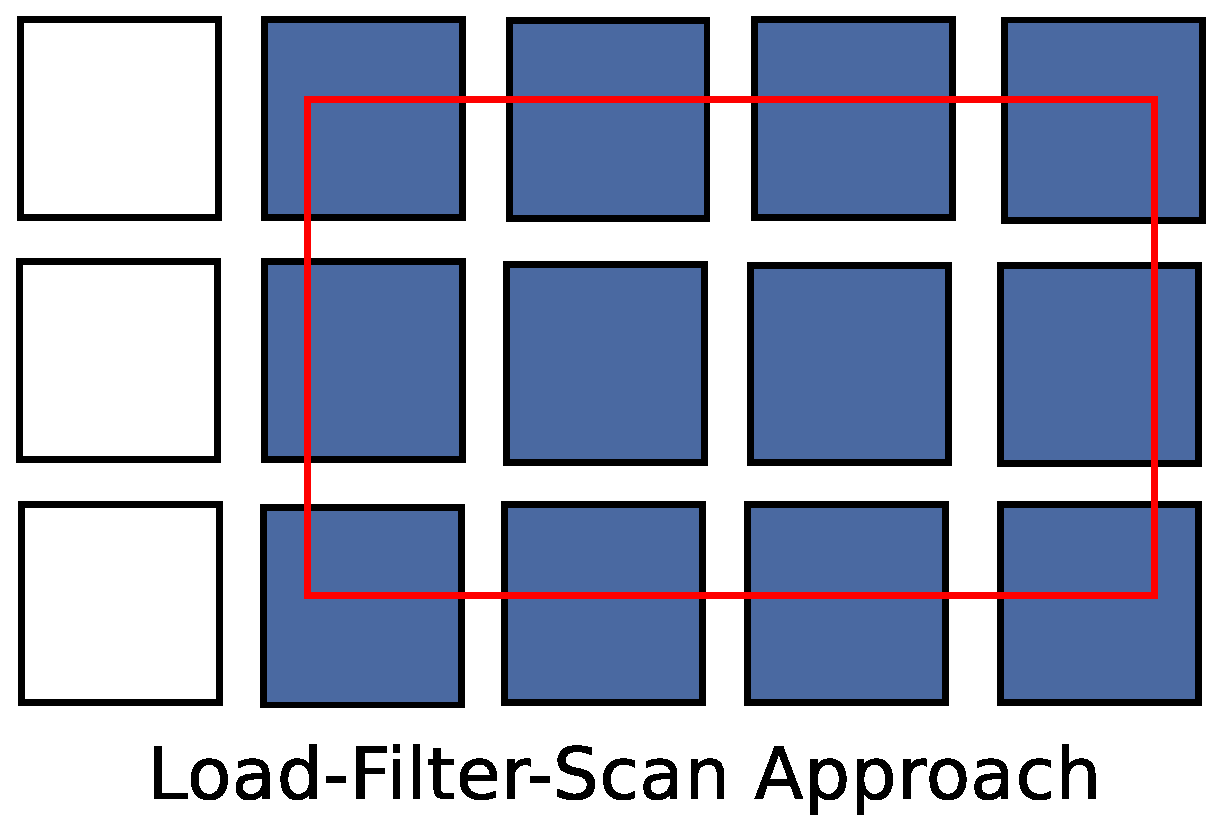
\includegraphics[width = 0.45\linewidth, keepaspectratio = true]{images/eps/loadfilterscan.eps}%}
	~
	%\subfloat[]{\label{fig:ih_mainbenefit}
	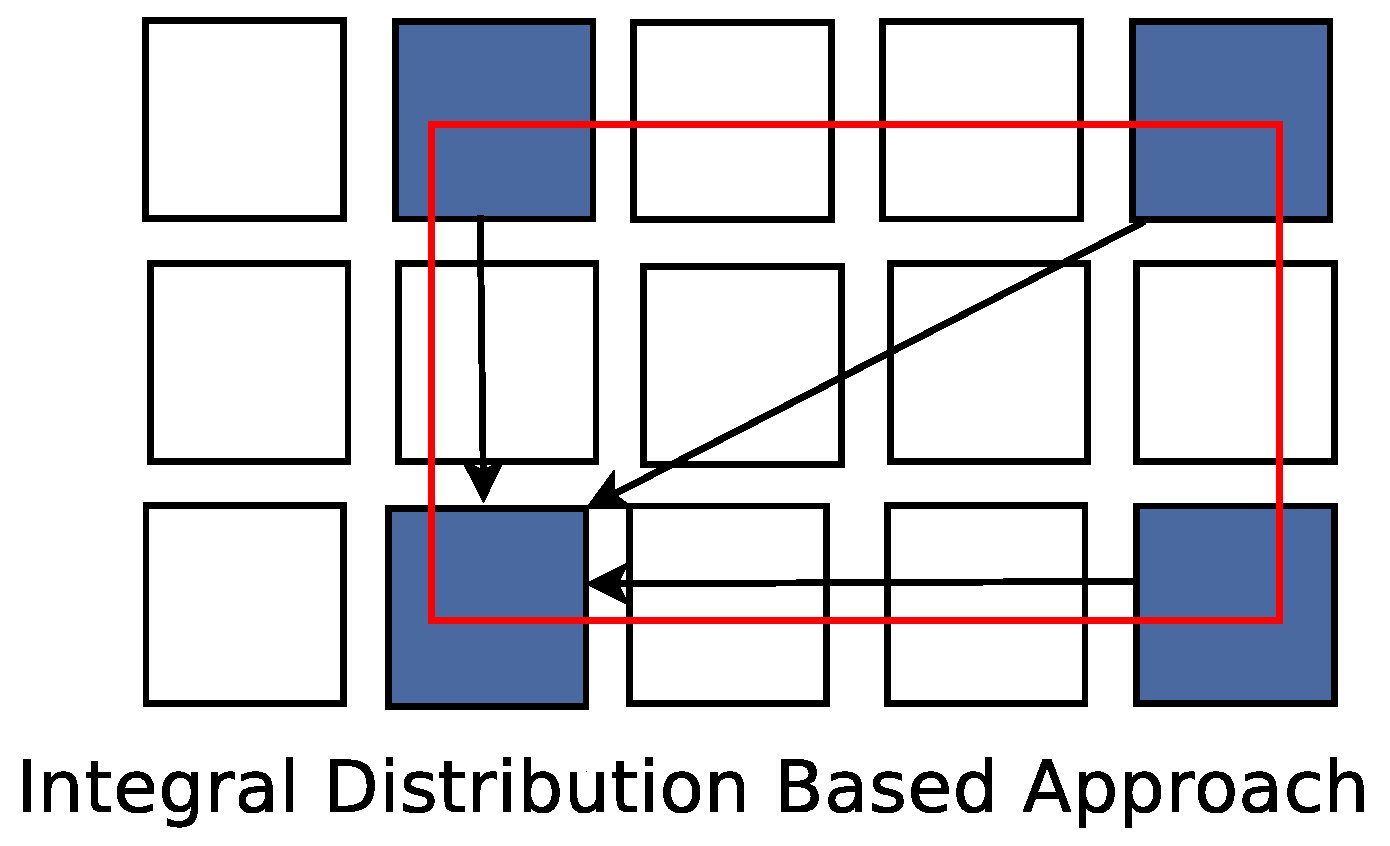
\includegraphics[width = 0.49\linewidth, keepaspectratio = true]{images/eps/mainbenefit.eps}%}
	\caption{{\bf Left.} Traditional raw data access method of answering range distribution queries where compute time, i/o and communication time are functions of query size. The blocks to be loaded to answer a query (red rectangle) are shaded in blue. {\bf Right.} Proposed integral distribution approach only needs to probe the 4 (8 in 3D) corners of a query region to answer it. Query response time is fixed regardless of query size.}	
	\label{fig:ih_mainbenefit}
\end{figure}
%%%%%%%%%%%%%%%%%%%%
%% Diagram ends
%%%%%%%%%%%%%%%%%%%

Our framework offers the ability to answer such a range distribution query in constant cost (in terms of computation time, I/O and/or communication cost), regardless of the query region size. As outlined in Figure~\ref{fig:ih_mainbenefit} (right), our framework can answer any query by probing only the $2^d$ corner points (8 for 3D) of a $d$-dimensional query. Hence, the I/O cost is bounded by that of 8 blocks and at most 8 communications are needed.

To give an overview, our framework, outlined in Figure~\ref{fig:ih_overview}, transforms the raw data into a data structure called Integral Distribution Volume (IDV). Since direct computation of IDV is slow and space-consuming for large data, we propose a scheme to compute the integral distribution of any location from a hierarchy of reusable block-level distributions. The high storage cost associated with IDV is reduced by applying a template-based encoding technique on the block-level distributions. Also, we allow the user to trade accuracy for speed by selectively using or discarding block-level distributions while answering query.
%%%%%%%%%%%%%%%%%%%
%% Diagram begins
%%%%%%%%%%%%%%%%%%%
\begin{figure}[tb]
\centering
	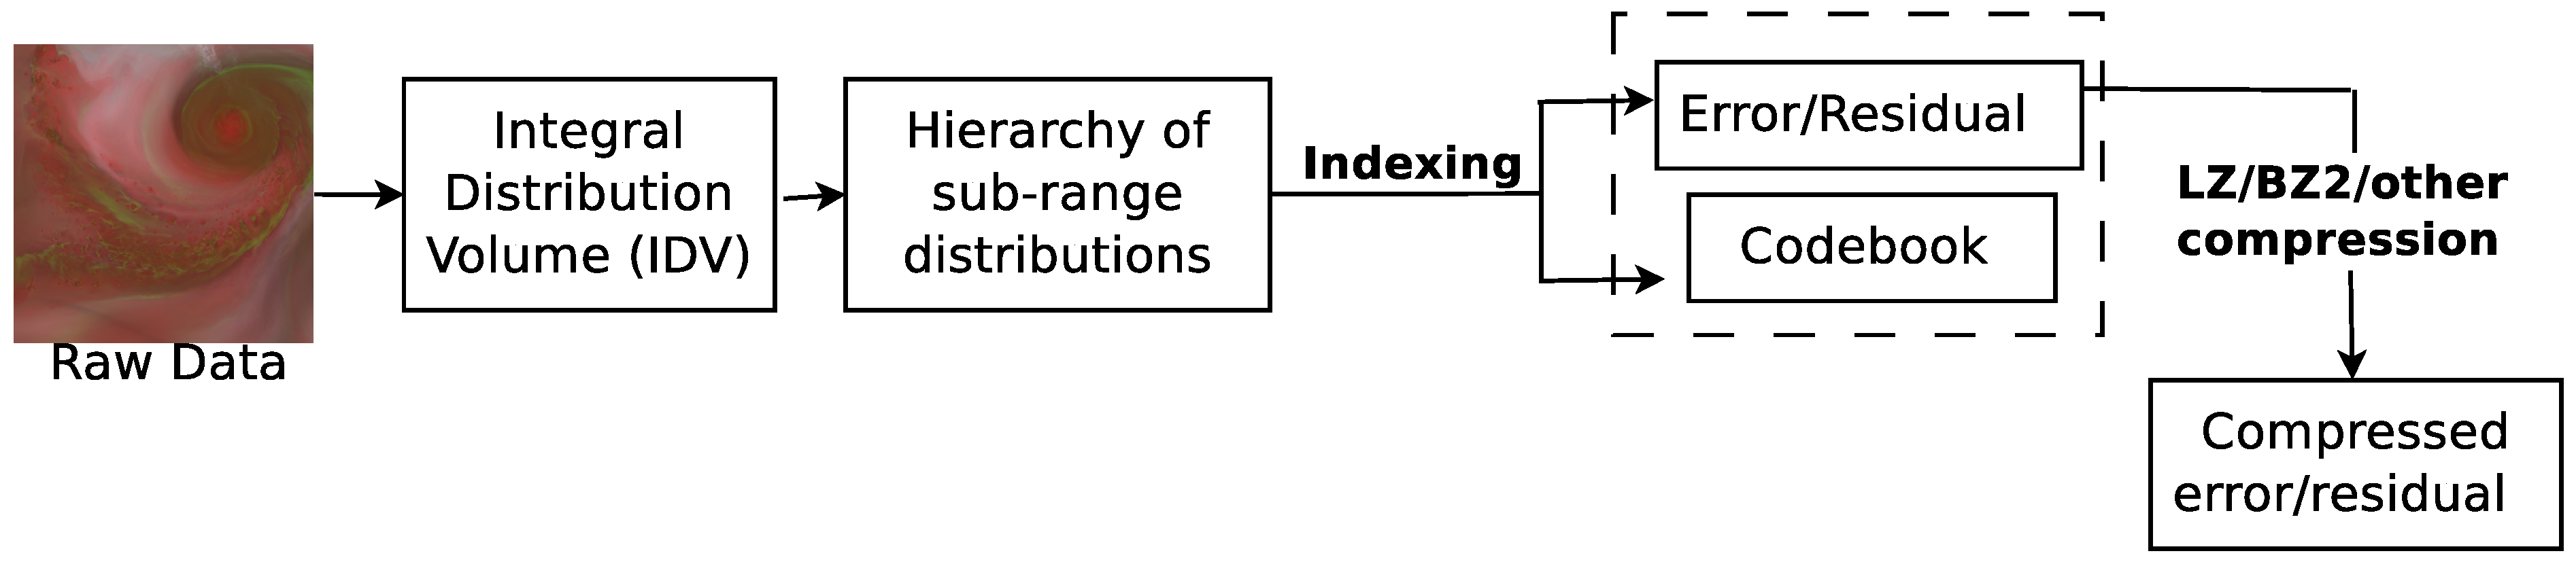
\includegraphics[width = \linewidth, keepaspectratio = true]{images/eps/overview.eps}
	\caption{Overview of the proposed framework for transformation and storage of integral distribution volume.}	
	\label{fig:ih_overview}	
\end{figure}
%%%%%%%%%%%%%%%%%%%%
%% Diagram ends
%%%%%%%%%%%%%%%%%%%

Our proposed framework is explained in following stages: representation of integral distribution by power-of-two lengths sub-range distributions, indexing of these sub-ranges followed by compression, and finally, interactive retrieval and reconstruction of range distributions. 
%%
%%
\subsection{Integral Distribution Volume (IDV)}
\label{subsec:ih_def}
%%
%%
Given an $N_x\times N_y\times N_z$ 3D field $f:R^3\to R$, its integral volume $I_f$ stores at each location the aggregate of the attribute value from origin to that location. Mathematically speaking, 
%%
\begin{align*}
I_f &= \{ I_f(x,y,z) : x\in [1,N_x], y\in [1,N_y], z\in [1,N_z]\}\text{, where}\\
I_f(x,y,z) &= \sum_{k=1}^{z}\sum_{j=1}^{y}\sum_{i=1}^{x} f(x, y, z) 
\end{align*}
%%
In other words, the integral volume stores the range prefix sums of $f$ at each data point. As a result, the aggregate of $f$ over any range $Q$ can be obtained by a finite number of addition and subtractions of the prefix sums at the corners of $Q$~\cite{SAT84, integhist05}. 

Integral Distribution Volume is an extension of the above idea to histograms. Given an $N_x\times N_y\times N_z$ 3D field, its \emph{integral distribution volume (IDV)} stores at each location the integral histogram, which is the distribution of the sub-field spanning from the origin to that location. The IDV of a volume under $K$-bin histogram representation is defined as:
%%
\begin{align*}
IDV_f&= \{ H(x,y,z) : x\in [1,N_x], y\in [1,N_y], z\in [1,N_z]\}\text{, where}
\end{align*}
%%
$H(x,y,z)$ denotes the integral histogram at $(x,y,z)$. The distribution of any 1D range $[A, B]$, denoted by $h([A, B])$, is obtained by using the integral distributions $H(A)$ (same as $h([1, A])$) and $H(B)$ (same as $h([1, B])$): $h([A, B]) = H(B) - H(A)$. In higher dimensions, the query is defined by more than two points (4 points in 2D, 8 in 3D for example). Hence, the distribution of a $d$-dimensional query range $\{A_i:i=[1,2^d]\}$ is retrieved by the following steps: $H(A_i)$ for each corner point $A_i$ are accessed from IDV; $H(i)$s are added or subtracted to obtain $h(\{A_i:i=[1,2^d]\})$. 
%%
%%
\subsection{Transformation to Sub-range Distributions}
\label{subsec:ih_decomp}
%%
%%
%%%%%%%%%%%%%%%%%%%
%% Diagram begins
%%%%%%%%%%%%%%%%%%%
\begin{figure}[tb]
\centering
	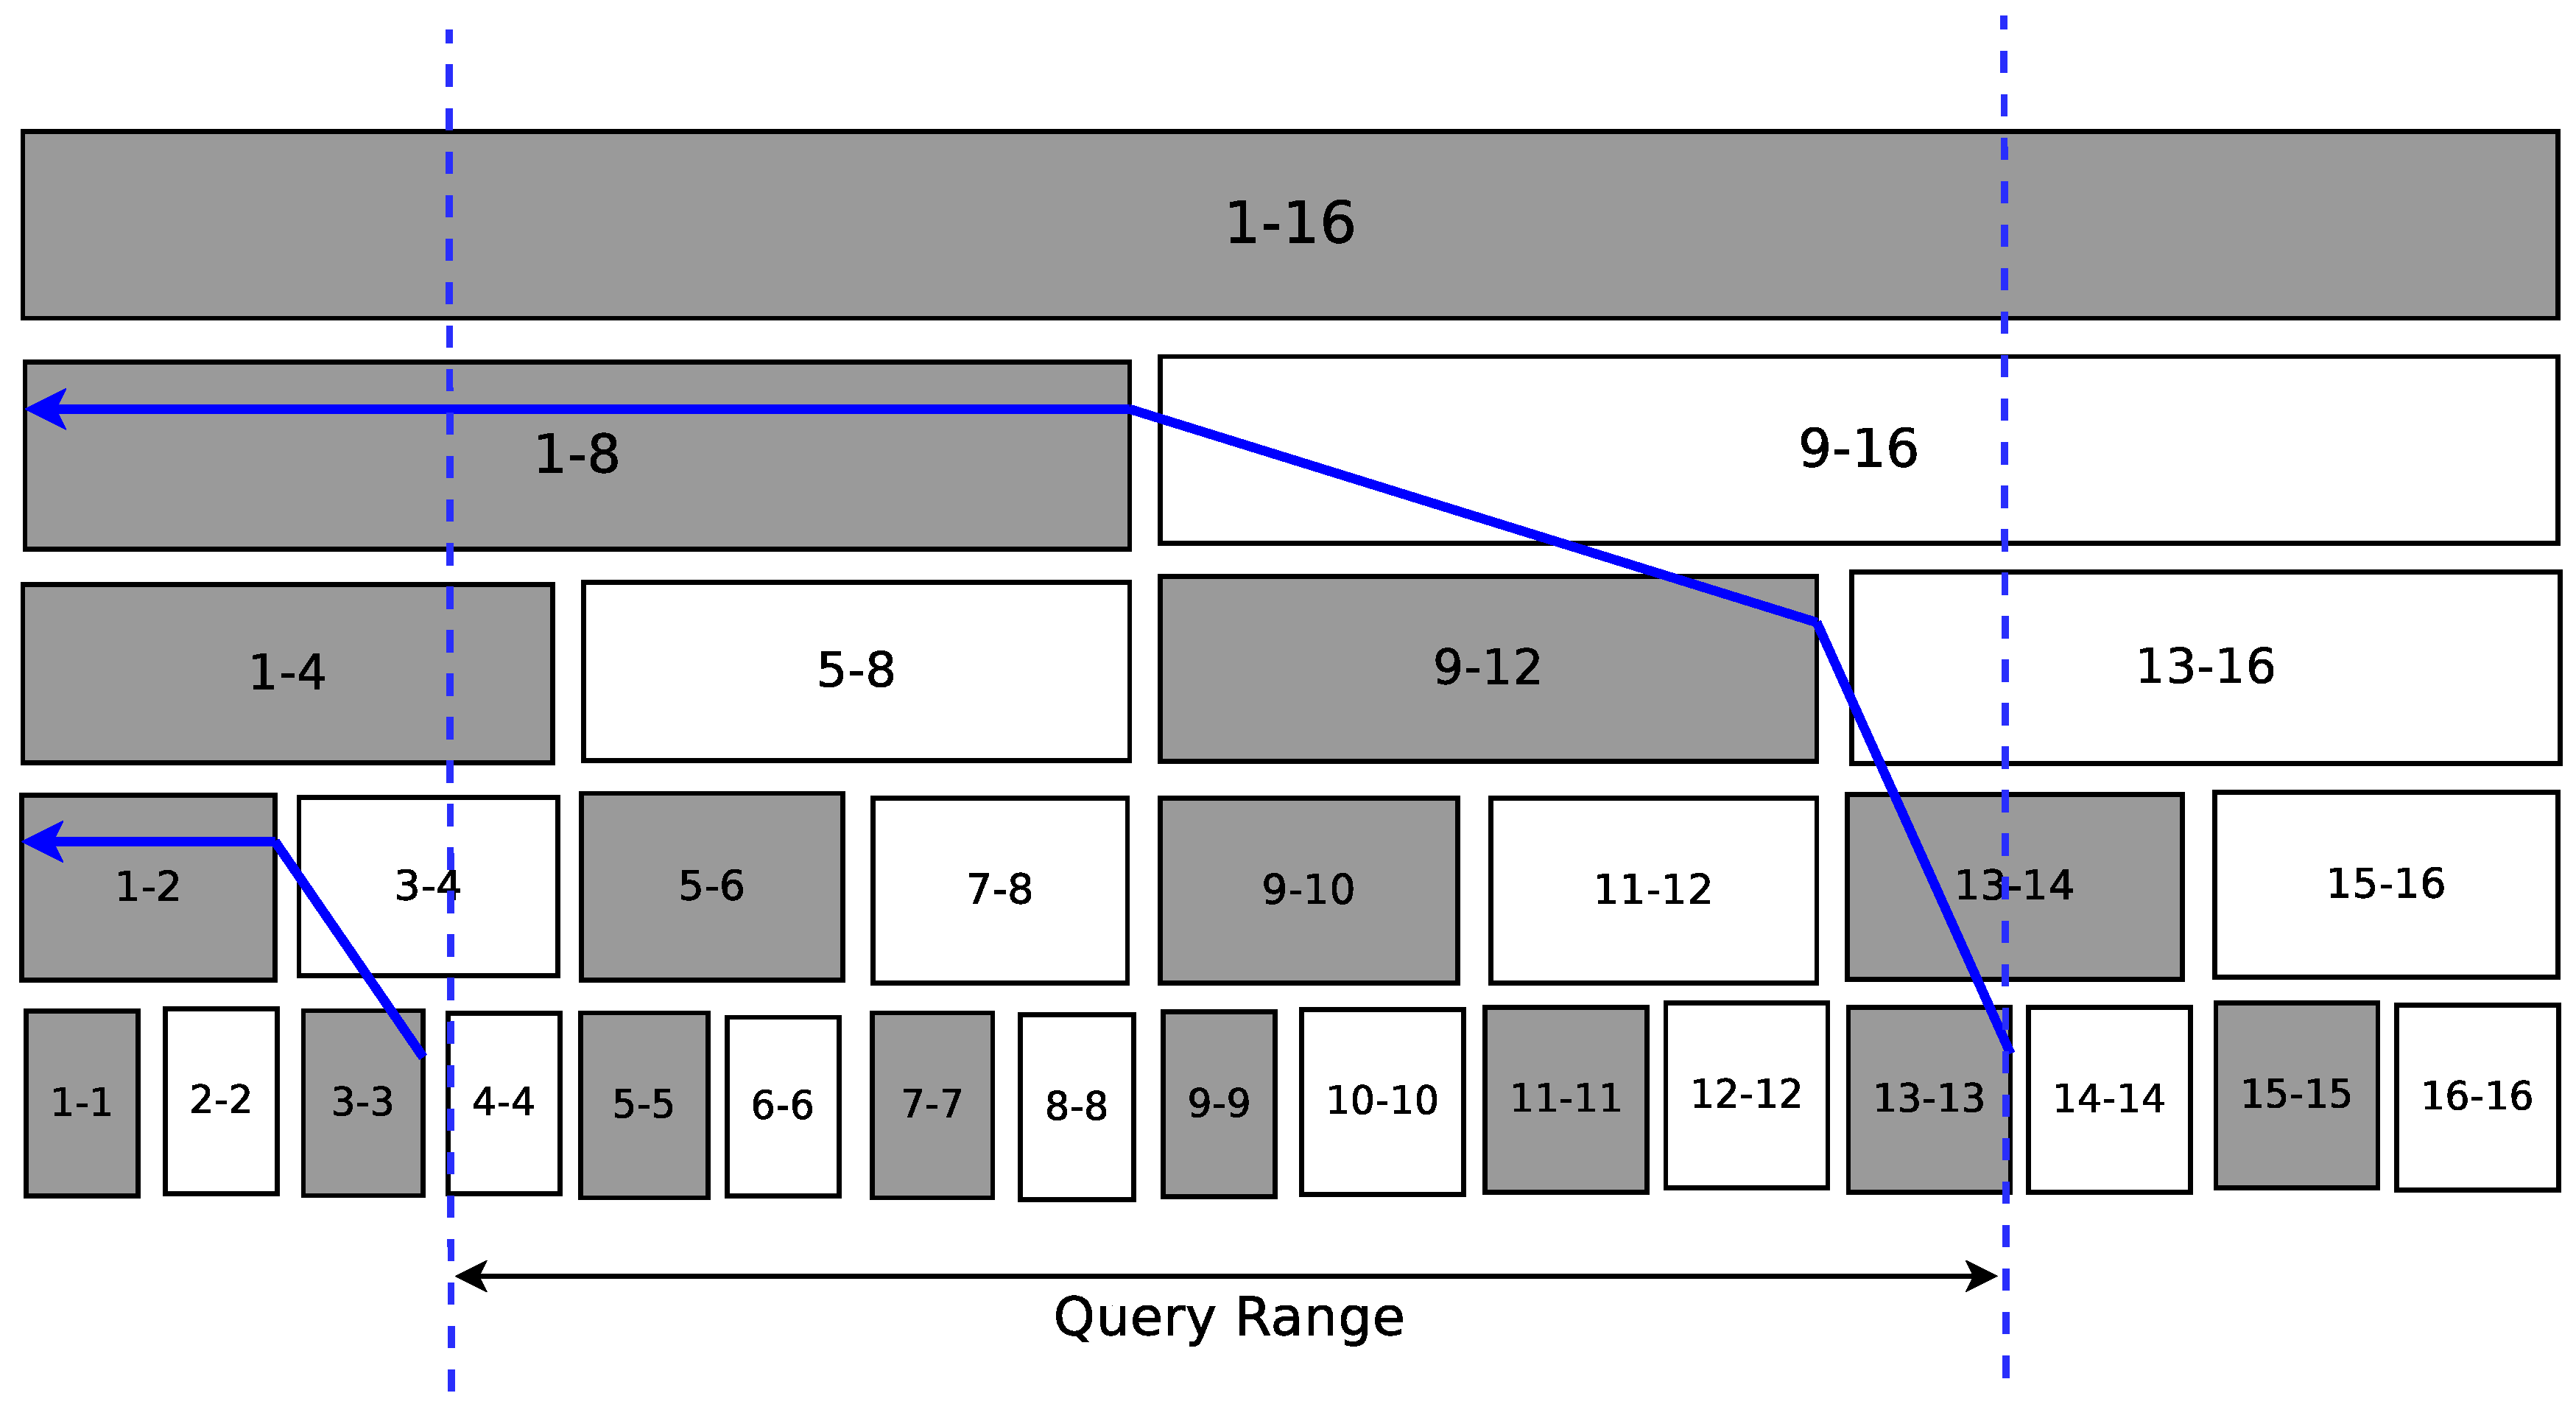
\includegraphics[width = \linewidth, keepaspectratio = true]{images/eps/ih_octree_ih.eps}
	\caption{Transformation of a 1D integral distribution. Only the distributions of the ranges colored in gray are sufficient to construct the distribution of any arbitrary range.}	
	\label{fig:ih_octree}
\end{figure}
%%%%%%%%%%%%%%%%%%%
%% Diagram ends
%%%%%%%%%%%%%%%%%%%
%%
The benefit of fixed computation cost of IDV comes at the cost of huge storage cost - $O(N_x\times N_y\times N_z\times K)$. Instead of directly applying an off-the-shelf compression to IDV, we propose to first decompose it into a number of sub-ranges and their distributions for two reasons:
%%
\begin{packed_itemize}
%%
\item These sub-range distributions can be repeatedly used to reconstruct the integral distribution at any location on the IDV
\item Compressing the sub-range distributions leads to more space-saving than directly compressing the IDV
%%
\end{packed_itemize}
%%
%%
The steps of decomposition are given below. We observe that given any 1D point $P$, the integral distribution $H(P)$ can be computed by combining $\log_2 P$ or less number of sub-range distributions from $[1,P]$, where each sub-range has a power-of-two length. Suppose, $S(P) = \{p_1, p_2, \ldots, p_n\}$ denotes the set of power-of-two sub-ranges for a point $P$. Given $P$, we obtain $S(P)$ using the following algorithm based on fast bitwise operation:
%%
\begin{packed_enumerate}
%%
\item The rightmost non-zero bit of the binary representation of $P$ is set to zero to obtain $P'$ ($P'<P)$
\item $[(P'+1),P]$ is stored as the next sub-range, $S(P) = S(P-P') \bigcup [(P'+1),P]$
\item Steps 1 and 2 are recursively applied on the residual, $(P-P')$
\item The recursion stops when $P'=0$
%%
\end{packed_enumerate}
%%
Figure~\ref{fig:ih_dcomp_algo} demonstrates the process with $P=25$. In 1D, each such sub-range comes from a binary tree which partitions the range $[1,P]$ (Figure~\ref{fig:ih_octree}). When $P$ is a higher dimensional point, the 1D blocks for each of its dimensions are first computed. Then, another iteration is performed to combine them into a set of higher dimensional power-of-two length blocks. Hence, $S(P(x,y,z)) = S(x)\times S(y)\times S(z)$.
%%
%%%%%%%%%%%%%%%%%%%
%% Diagram begins
%%%%%%%%%%%%%%%%%%%
\begin{wrapfigure}{R}{0.5\linewidth}
\centering
	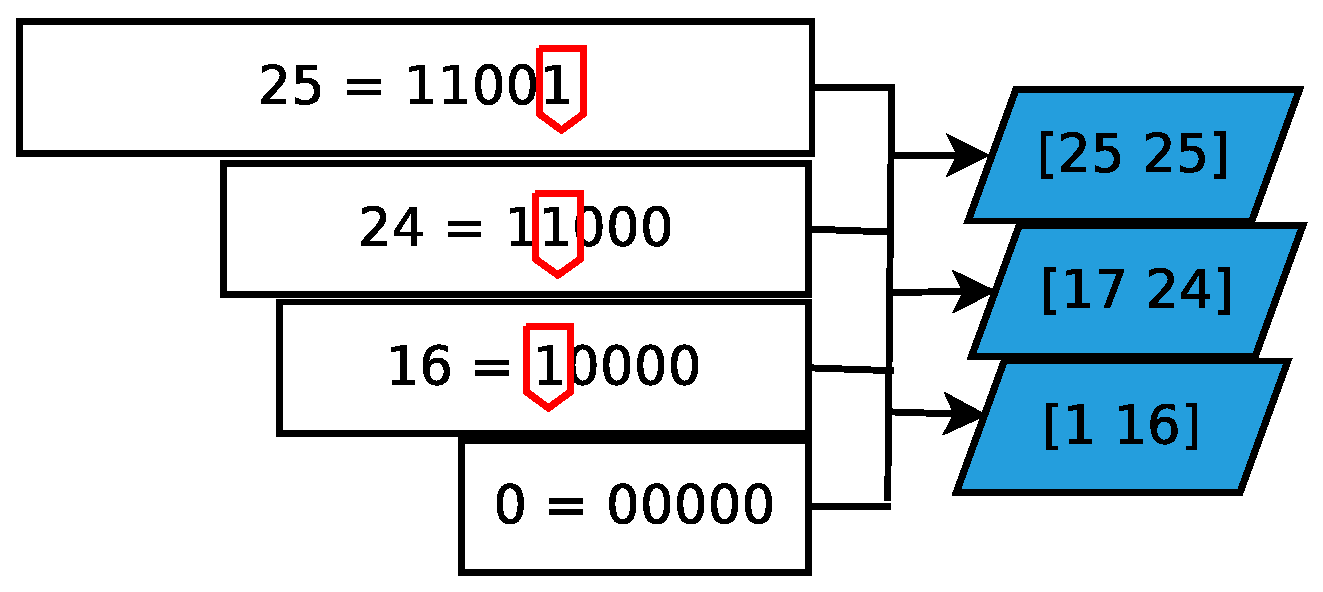
\includegraphics[width = \linewidth, keepaspectratio = true]{images/eps/decomp_algo.eps}
	\caption{Fast algorithm to decompose a range into power-of-two length blocks.}	
	\label{fig:ih_dcomp_algo}
\end{wrapfigure}
%%%%%%%%%%%%%%%%%%%
%% Diagram ends
%%%%%%%%%%%%%%%%%%%

Integral distributions of nearby points share blocks among them. For example, $S(4)$ contains $[1,4]$, which also appears in $S(5)$ which is $\{[1,4],[5,5]\}$ and $S(6)$ which is $\{[1,4],[5,6]\}$. Hence, after running the above algorithm for entire range from 1 to $P$, we discard the duplicate blocks and retain the union of all minus the duplicates. In 1D, it turns out that storing every alternate sub-range at each level of the binary tree is sufficient to reconstruct $H(P)$ for any arbitrary $P$. Figure~\ref{fig:ih_octree} shades the blocks which are sufficient to reconstruct any integral distribution in 1D. The principle holds in 2D or 3D as well. 

Hence, the first transformation of IDV creates a set containing same number of sub-range distributions as the IDV does. However, these sub-range distributions are non-integral, and hence can be computed much faster. More importantly, most sub-ranges represent small spatial regions (half of them only contain 1 data point), and are likely to have a very small number of non-zero bins. So they can be stored much more compactly and lend themselves more easily to various compression schemes. When we need to store non-normalized distributions, the range of frequencies of the sub-range distributions is much smaller compared to the original integral distributions. This also leads to better compression.  
\subsection{Indexing of Sub-Range Distributions}
\label{sec:blockhist_coding}
%%
We propose to index the sub-range distributions in such a way that the indexed distributions lead to even more space saving under any standard compression algorithm. In essence, the set of sub-range distributions, denoted by $B$, is indexed by a much smaller set of template distributions, denoted by $T$, which represents different types of distributions in the dataset. The proposed algorithm finds a mapping $\Theta: B \to T$ from each element $h_i(B)$ of $B$ to one or more elements of $h_j(T)$ of $T$. At the end, $B$ is discarded; only the map and the template set is retained. Since $B>>T$, this reduces the storage cost. In the query phase, the required elements of $B$ are approximated using the map and their images in $T$. Figure~\ref{fig:indexing_overview} presents a schematic overview of the indexing algorithm.
%%
%%%%%%%%%%%%%%%%%%%
%% Diagram begins
%%%%%%%%%%%%%%%%%%%
\begin{figure}[tb]
\centering
	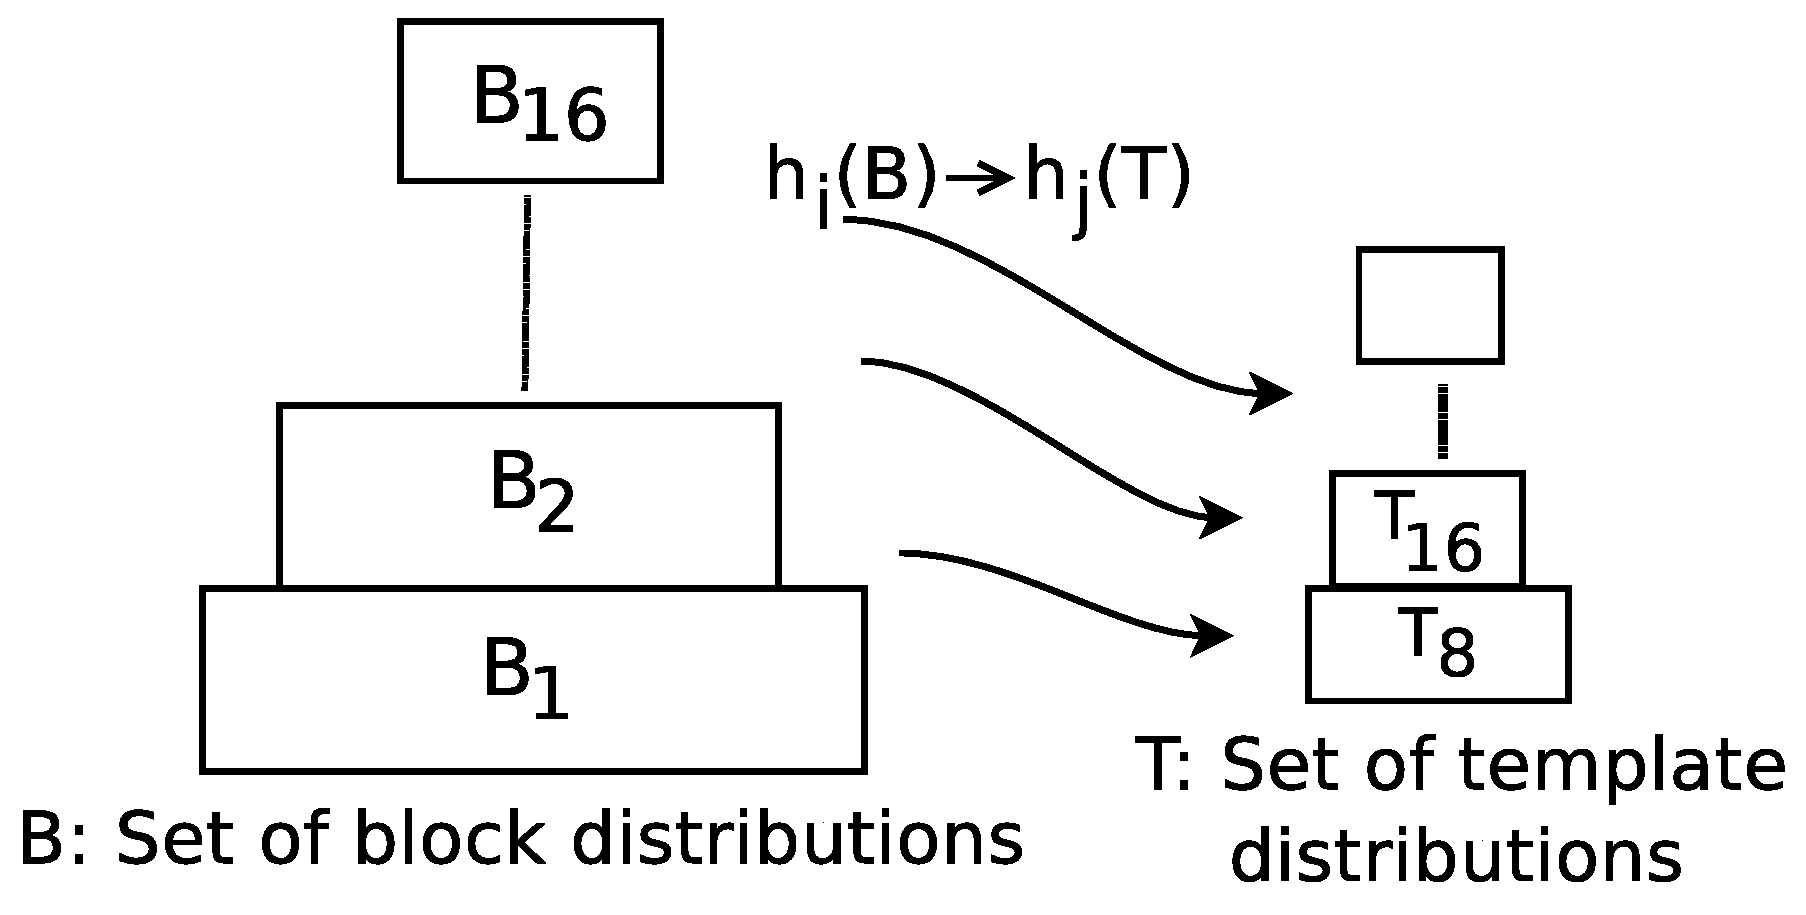
\includegraphics[width = 0.55\linewidth, keepaspectratio = true]{images/eps/indexing.eps}
	\caption{Overview of the indexing algorithm, where sub-range distributions, grouped based on their sizes, find an approximate match from a much smaller set of template distributions.}	
	\label{fig:indexing_overview}	
\end{figure}
%%%%%%%%%%%%%%%%%%%%
%% Diagram ends
%%%%%%%%%%%%%%%%%%%

A template based indexing performs well if the elements of $B$ are similar to each other so that many of them are indexed to one template. This reduces the number of elements to retain from $T$ and hence, reduces the total storage cost. In our case, the created sub-range distributions can be grouped based on the sizes of the blocks they come from, as shown by $B_1$, $B_2$ etc. in Figure~\ref{fig:indexing_overview}. The distributions of any given group $B_i$ are more likely to be similar to each other, which makes them easier to index against a certain type of templates. An integral distribution volume in its original form would not offer this benefit, since every distribution would come from a different-sized block. The steps of the indexing algorithm are described below. 

%%
%%
\subsubsection{Construction of Templates}
\label{subsec:templateconstruction}
%%
%The proposed algorithm works under the assumption that the data has redundancy and every feature (in our case distribution) has multiple copies in the data. Under this assumption, even if we select a few templates via regular sampling of the spatial domain, the likelihood of every type of distribution being selected at least once is high. This assumption also precludes the need to use expensive clustering methods for template creation, and hence suits large-scale data.
%%
%%%%%%%%%%%%%%%%%%%
%% Diagram begins
%%%%%%%%%%%%%%%%%%%
%\begin{figure}[tb]
%\centering
%	\includegraphics[width = 0.35\linewidth, keepaspectratio = true]{images/eps/templates_stratified.eps}
%	\caption{{\bf *** FIGURE WILL CHANGE ***}Proposed strategy for template creation. In this example, $H(P_1), \ldots H(P_9)$ - the normalized integral histograms at the sampled points - constitute the set of templates.}	
%	\label{fig:templatecreation}
%\end{figure}
%%%%%%%%%%%%%%%%%%%
%% Diagram ends
%%%%%%%%%%%%%%%%%%%

In our formulation, the distributions to be encoded (set $B$) come only from power-of-2 length blocks. This is why we create a similar structured yet much smaller set of templates $T$ from power-of-2 length blocks obtained from a downsampled copy of the data. Spatially smoothed downsampled data is used so that the local features and noises do not bias the templates. The templates are created using the following steps:
%%
\begin{packed_enumerate}
%%
\item The data is downsampled by one level using a standard spatial smoothing technique. We have an empty set $T$.
\item The downsampled data domain is decomposed into non-overlapping partitions of length $b$ where $b$ is a power of two. We have started with 4 as the initial value of $b$. 
\item Every $k$-th partition along each dimension is selected (where $k$ denotes stride) and its distribution is included in a set $T_b$
\item $T = T \bigcup T_b$
\item $b = 2\times b$ and $k = max \{k/2, 1\}$. Steps 2 and 3 are repeated with a bigger partition and a smaller stride. This is done until partition size is nearly half as the domain
%%
\end{packed_enumerate}
%%
This algorithm produces $T$ only from power-of-two blocks of different sizes. This makes it fit for indexing the hierarchy of block distributions $B$. Even though a sub-range distribution is free to index against any template coming from any region in the spatial domain, it is more likely to find a match from the subset coming from sub-ranges of equivalent size in the downsampled data. 
%%
%%
\subsubsection{Mapping Distributions to Templates}
\label{subsec:encoding}
%%
The next step is to create the map $\Theta: B\to T$. For each block histogram, the goal is to find a template which best approximates it. However, since $|T|<<|B|$, a block histogram may not find a good match in $T$. Thus, given an input block histogram, each template undergoes a set of transformations to virtually expand the set of templates available for each block. The proposed indexing can be expressed as following:
%%
\begin{align*}
\Theta(h_i(B)) = \{ j, \tau \}
\text{, if } \Delta(h_i(B),\tau(h_j(T)) \text{is minimum} \forall j
\end{align*}
%%
where $\tau$ represents the transformation of a template and $\Delta(a,b)$ represents the difference between histograms $a$ and $b$, 
%%
%%%%%%%%%%%%%%%%%%%
%% Diagram begins
%%%%%%%%%%%%%%%%%%%
\begin{figure}[tb]
\centering
	\subfloat[Intuition behind circular shift and reflection.]{\label{fig:histtransformreason}
	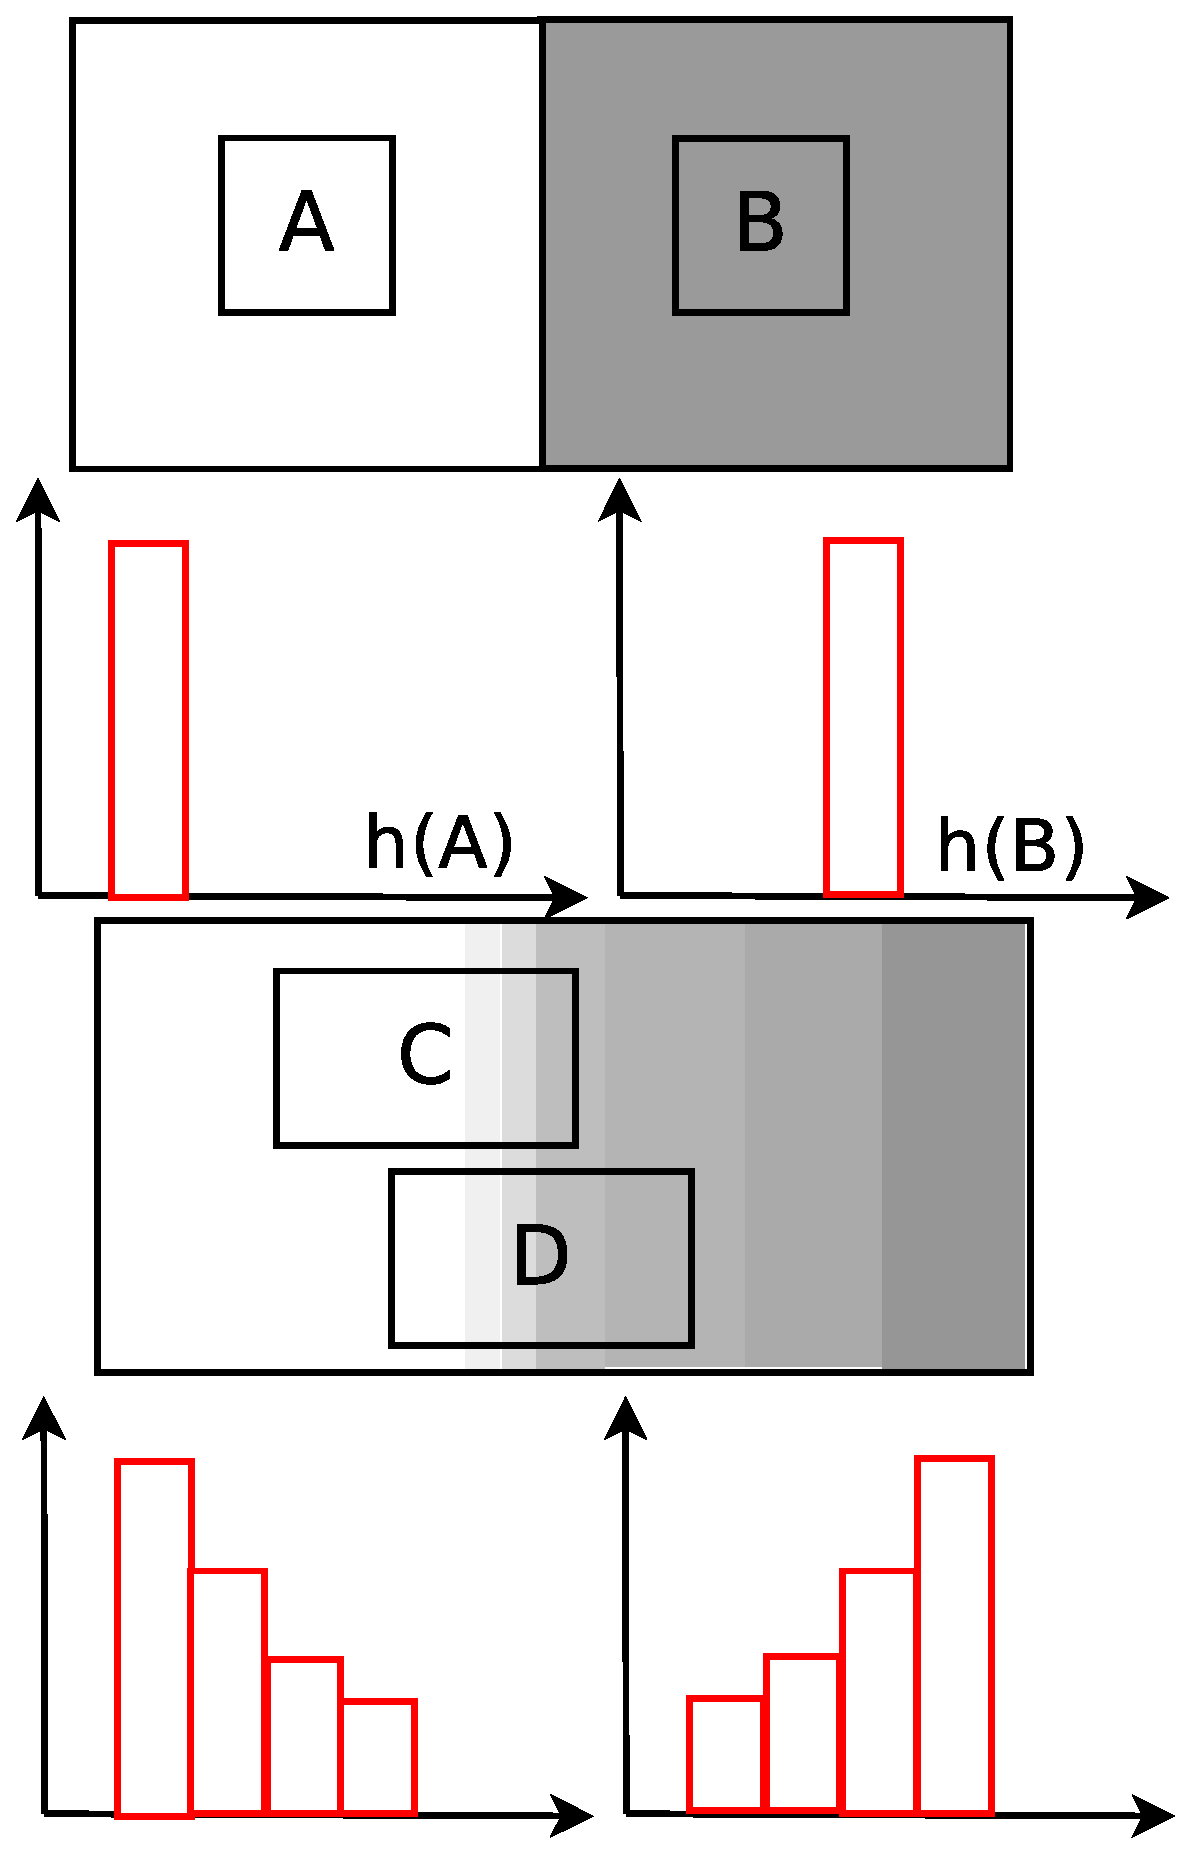
\includegraphics[width = 0.3\linewidth, keepaspectratio = true]{images/eps/histtransform_justification.eps}}
	~
	\subfloat[Peak matching followed by local alignment]{\label{fig:histtransformdetail}
	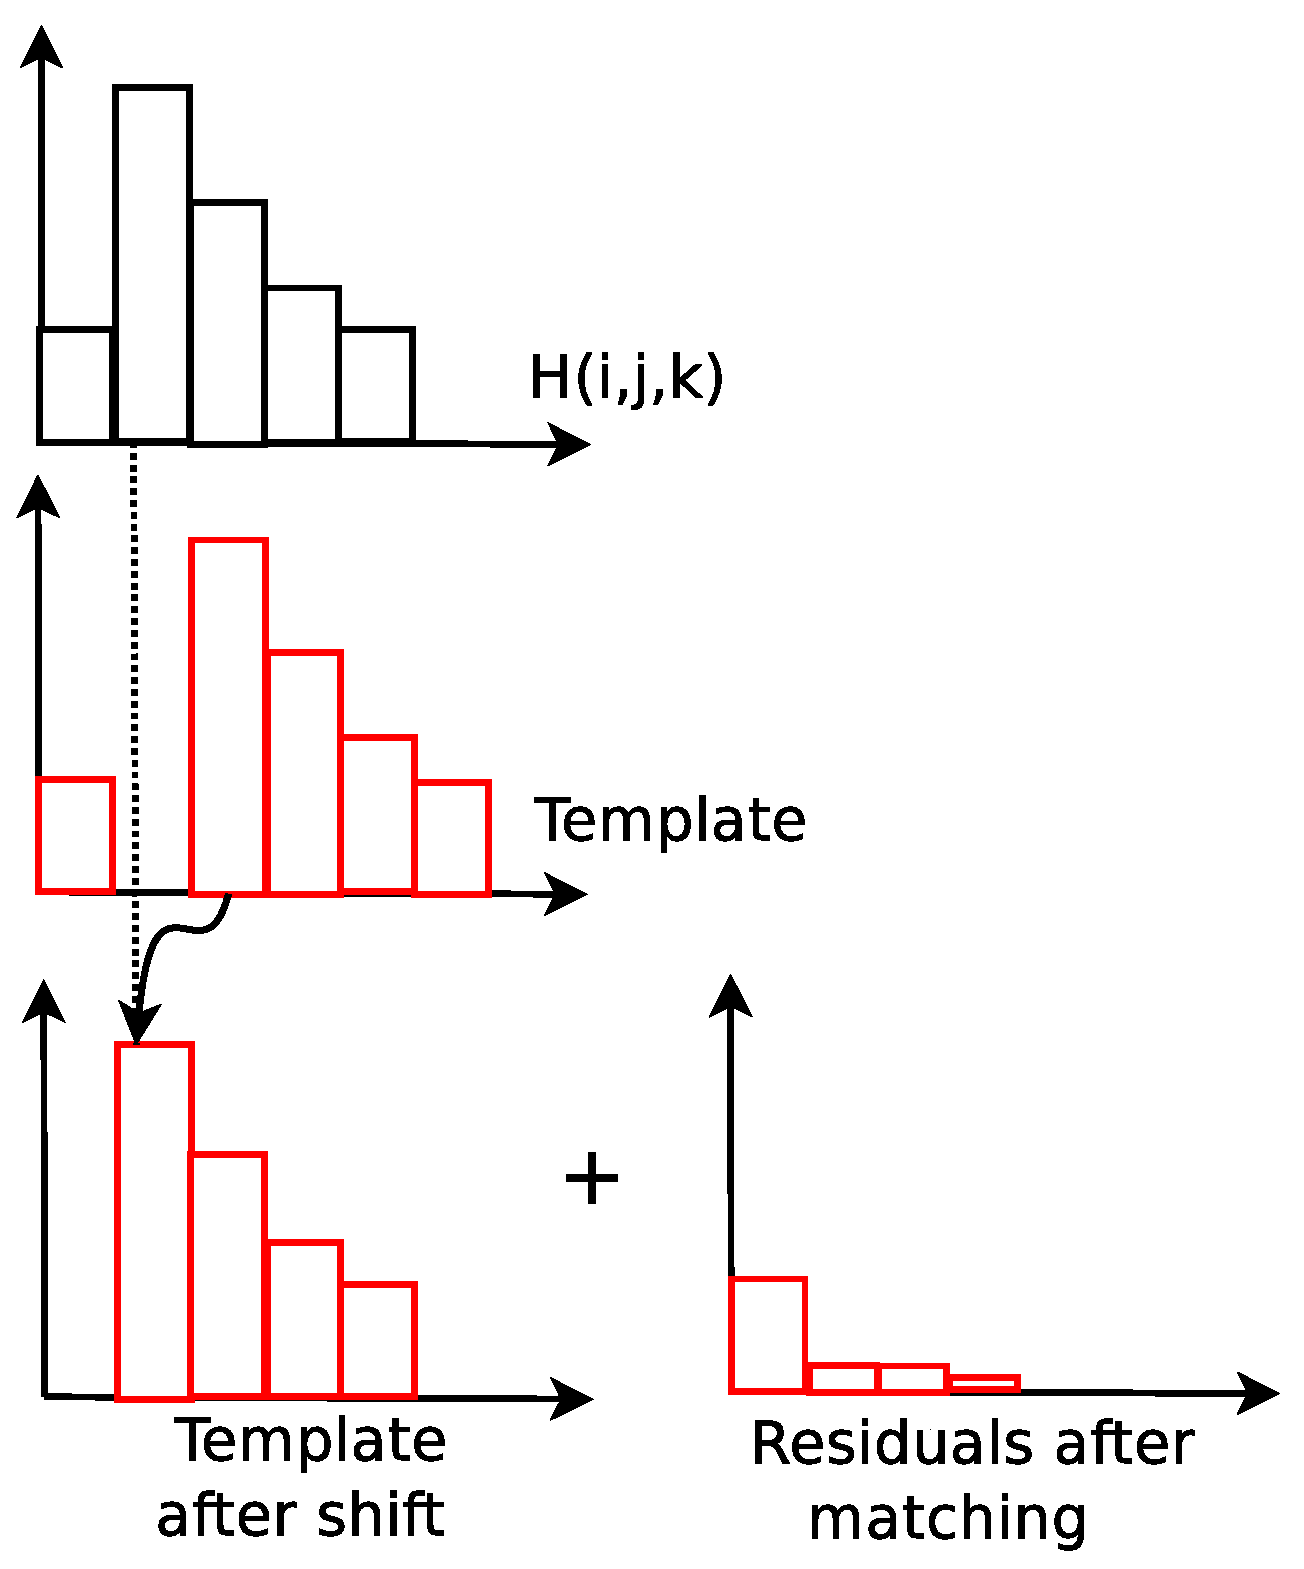
\includegraphics[width = 0.4\linewidth, keepaspectratio = true]{images/eps/histtransform_fast.eps}}
	\caption{(a) Schematic presentation of chosen transformations for histograms. (b) Fast implementation of shift and reflection through  peak matching and local adjustment.}	
	\label{fig:histtransform}
\end{figure}
%%%%%%%%%%%%%%%%%%%
%% Diagram ends
%%%%%%%%%%%%%%%%

We match histogram shapes by detecting corresponding points, which are the bin centers for a pair with same number of bins, and then transforming one to align the correspondent points. We observed that \emph{circular shift} and \emph{reflection} form a suitable set of aligning transformations. These two capture all possible shifts of the bins, while preserving the relative order. The intuition behind choosing these transformations is as follows:
%%
\begin{packed_itemize}
%%
\item Circular shift corresponds to change of location in the data space. In a volume data composed of multiple materials, when we move from one uniform zone $A$, made of one material, to another zone $B$ made of a different material, the data values shift and so does the histograms ($h(A)$ shifts to $h(B)$ as in Figure~\ref{fig:histtransformreason}). 
%%
\item Data sets also contain regions with gradually changing values. Change of location in such regions corresponds to reflection of histograms. For example, in Figure~\ref{fig:histtransformreason}, the histograms of $C$ and $D$ can be transformed though reflection followed by translation.
%%
\end{packed_itemize}
%%%
In case of a 1D histogram, the shifts are produced by shifting every bin to its right by one step at each iteration. The rightmost bin is circularly brought back to the leftmost bin. Then, if necessary, the histogram is reflected so that for each $i$, $f(i)$ becomes $f(K-i)$. Then $K$ circular shifts are applied on the reflected histogram. Instead of exhaustively matching against all shifted positions, we first align them by their mode (bin with highest frequency), and then shift the template only by a small number of steps in both directions ( Figure~\ref{fig:histtransformdetail} right). 

Under each of these transformations, the transformed template histogram is compared against the block distribution under consideration. After the input has been compared with all templates and all transformations, the $<$\emph{template,transformation}$>$ pair leading to minimum error ($\Delta$) is remembered. In our case, transformation $\tau (h)$ involves two pieces of information: the amount or rotation $n_R$, and a boolean flag $b_R$ denoting if reflection is needed. We measure error by L-2 norm, which is $\Sigma_{i=1}^K d_i^2$, where $d_i$ represents the difference between the frequencies at $i^{th}$ bins of two histograms under consideration. We also store the \emph{residuals} - bin-wise frequency differences between the block distribution and template chosen for it. 
%% 
%%
\subsubsection{Compression of Indexing Results}
\label{subsubsec:compression}
%%
The output of the above two steps is a $<$\emph{template,transformation, residual}$>$ triplet for each block distribution. It may be noted that, due to indexing, each of the three information has become friendly to compression. The template id can take values only within the range 0 to $(|T|-1)$, which is not large. The rotation amount can vary only between 0 and $(K-1)$, if $K$ bins are used. The reflection flag is only 0 or 1. Most importantly, the residuals are more likely to have very small numbers since the chosen template has already been aligned against the block distribution. 

Hence, each of these information can be stored in separate files and compressed using any off-the-shelf compression technique. We have experimented with a few lossless compression schemes such as LZ~\cite{lz77} and bzip2. However, our work is not tied up to any particular compression technique, we have focused on increasing the compressibility of the data in general.  
\subsection{Range Distribution Query}
\label{subsec:query}
%%
%%
The main goal of the pre-processing described so far is to improve the performance of arbitrary range distribution queries (run by the user or an application) on large-scale datasets. The pre-processing makes the query phase lightweight and fast. 

To answer a range distribution query for region $Q$, we first obtain the integral distribution - $H(Q_i)$ - at each corner point $Q_i$ of the query. To get $H(Q_i)$, we need to access and de-compress the codebook of the block that contains $Q_i$. We subdivide the range $[1,Q_i]$ into a set of sub-ranges denoted by $S(Q_i)= \{q_1,q_2, . . . ,q_\}$ using the algorithm described before. Distribution for each $q_i$ is retrieved from the codebook. The decoding phase also requires the set of template distributions $T$ to be loaded. However, since $T$ is a small set, compressing it is not mandatory.
%%
%%%%%%%%%%%%%%%%%%%
%% Diagram begins
%%%%%%%%%%%%%%%%%%%
\begin{figure}[!htb]
\centering
	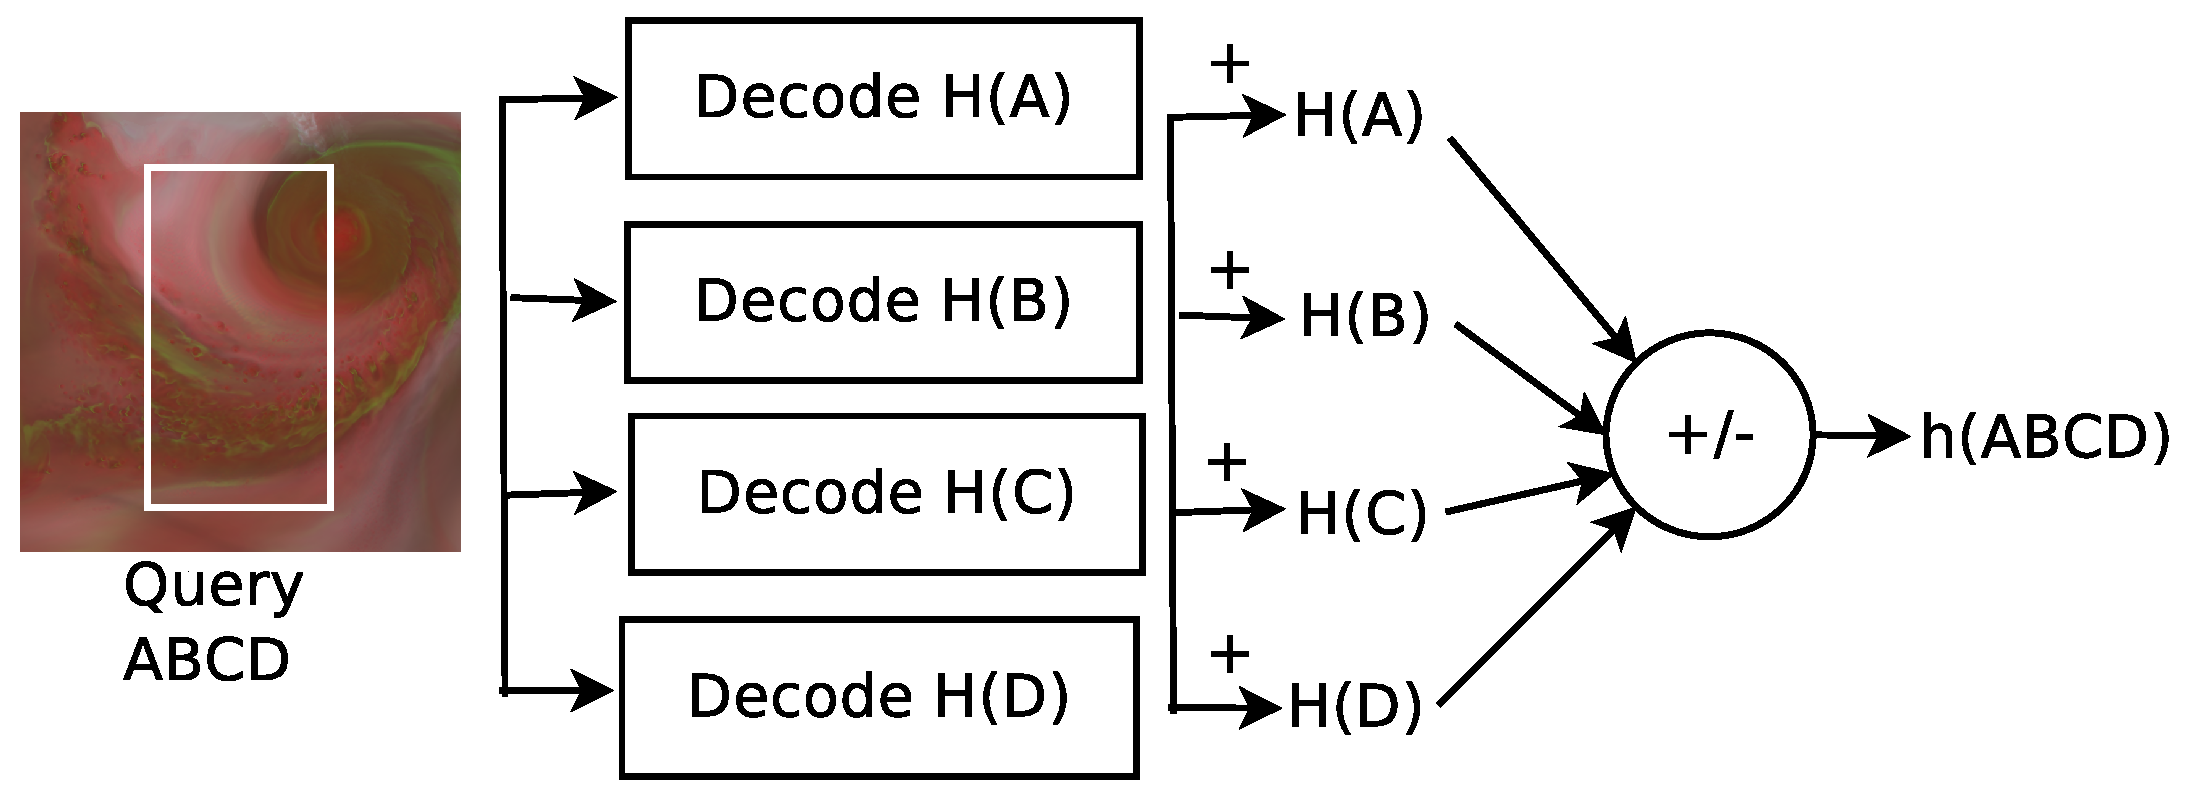
\includegraphics[width = 0.84\linewidth, keepaspectratio = true]{images/eps/decoding.eps}
	\caption{Retrieval of integral distribution at different locations requires to search the index tree up to different levels.}	
	\label{fig:retrieval}
\end{figure}
%%%%%%%%%%%%%%%%%%%
%% Diagram ends
%%%%%%%%%%%%%%%%%%%

Retrieval of a $h(q_j)$ from the codebook involves the following steps:
%%
\begin{packed_enumerate}
\item The codebook is used to retrieve the index to a template, say $k$ and a transformation $\tau$
\item Template histogram $h_k(T)$ is retrieved from template set $T$
\item The transformation is applied to the template histogram to obtain $\tau(h_k(T))$
\item The stored residuals $\delta$ for this mapping is retrieved, decompressed if needed, and applied to obtain $h(q_j) = \tau(h_k(T))+\delta$. 
\end{packed_enumerate}
%%
Addition of all $h(q_j)$s results in $H(Q_i)$, which eventually leads to $H(Q)$ (Figure~\ref{fig:retrieval}). 

Hence, our framework reduces the application workload in two ways. First, the query requires to access only eight corners, regardless of the query size. If the indexing results fit in memory, then it limits the memory access. If the indexing results for each data partition has been stored in compressed files, then it limits the number of disk accesses. Second, the retrieval of each corner distribution involves addition of a small number of spans, and then adding/subtracting corner histograms. Since the number of spans at any location $x$ is at most $\log x$, the computation required is much less compared to raw data scan, especially for large queries. Both of these lead to smaller query response time.
%%
%%
\remove
{
\subsection{Adaptations for Large Data}
\label{subsec:largedata}
%%
%%
%%%%%%%%%%%%%%%%%%%
%% Diagram begins
%%%%%%%%%%%%%%%%%%%
\begin{figure}[!htb]
\centering
	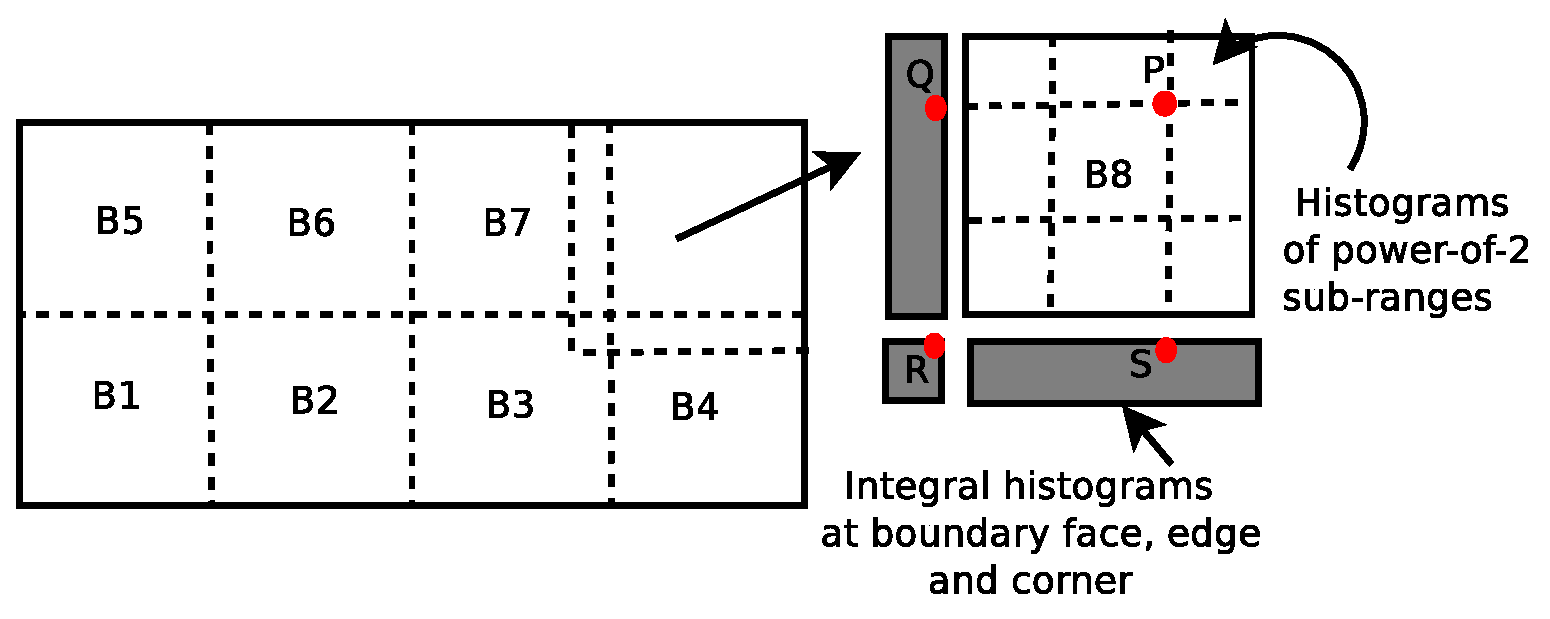
\includegraphics[width = 0.9\linewidth, keepaspectratio = true]{images/eps/ih_blockeddata.eps}
	\caption{Computing and encoding integral distributions from large data partitioned into blocks.}	
	\label{fig:blockeddata}
\end{figure}
%%%%%%%%%%%%%%%%%%%
%% Diagram ends
%%%%%%%%%%%%%%%%%%%
%%
%%
The benefit of such a framework is more clearly observed when the data is partitioned into blocks and distributed across many processors. In this section, we discuss a few adaptations which are necessary when applying this framework to partitioned data. 
%%
\begin{packed_itemize}
%%
\item Each data block simultaneously computes its own list of templates. A global list of templates is then created accumulating the local lists and the global list is distributed back to every block. A global list is used for indexing because even if two blocks are spatially far apart, they may contain similar distributions. 
\item Each data block is decomposed into power-of-two spans in its own local co-ordinates space. However, reconstructing these span distributions would not give back the global distribution of a corner point required for decoding. The global integral distribution at any point depends on its preceding blocks. Since speed is more important in the query phase, we pre-compute and store the integral distributions (in global coordinates space) for the corner point, three faces and three edges of the preceding blocks. Figure~\ref{fig:blockeddata} shows a 2D example where the integral distribution at point P in block B8 is computed from the spans and the pre-computed integral distributions at points Q, R and S.  
%%
\end{packed_itemize}
%%
}
 


%\input{sections/improvement.tex}
\section{Applications}
\label{sec:application}
%%
The proposed technique benefits any visualization application which implicitly runs range distribution queries on the data. Applications mainly run three types of distribution queries:
%%
\begin{itemize}
%%
\item \emph{Random:} Interactive exploration of the spatial domain by the user is an example which places queries in random locations and sizes in no particular order.
\item \emph{Blockwise:} Some applications partition the data into blocks and require the distribution of each block as a substitute of downsampled data. Examples which compute low resolution approximate isosurfaces~\cite{Hixel11} or streamlines from distributions, or visualizations that present blocks clustered by their distributions~\cite{transgraph11} fall in this category.  Blockwise queries become difficult to answer when the application (or the user) demands blocks of a different size.
\item \emph{Pointwise:} Many applications compute and analyze statistical properties such as mean, variance and information entropy~\cite{Xu10} from distributions computed based on a local neighborhood at each point. Computation of pointwise queries across large domains is expensive, since it requires raw data access, as the query range or the per-voxel neighborhood size is changed.
%%
\end{itemize}

Our method seamlessly integrates with any visualization application which falls in one or more of the above three categories. Instead of accessing the raw data to answer each query, we use our method to retrieve the distributions faster. Following two subsections show two such applications.
%%
%%
%%\subsection{Analysis of Local Statistics}
%%\label{sec:application_1}
%%
%%
%% 
%%
%%
%%%%%%%%%%%%%%%%%%%%%
%% Diagram begins
%%%%%%%%%%%%%%%%%%%
%\begin{figure}[!htb]
%\centering
%	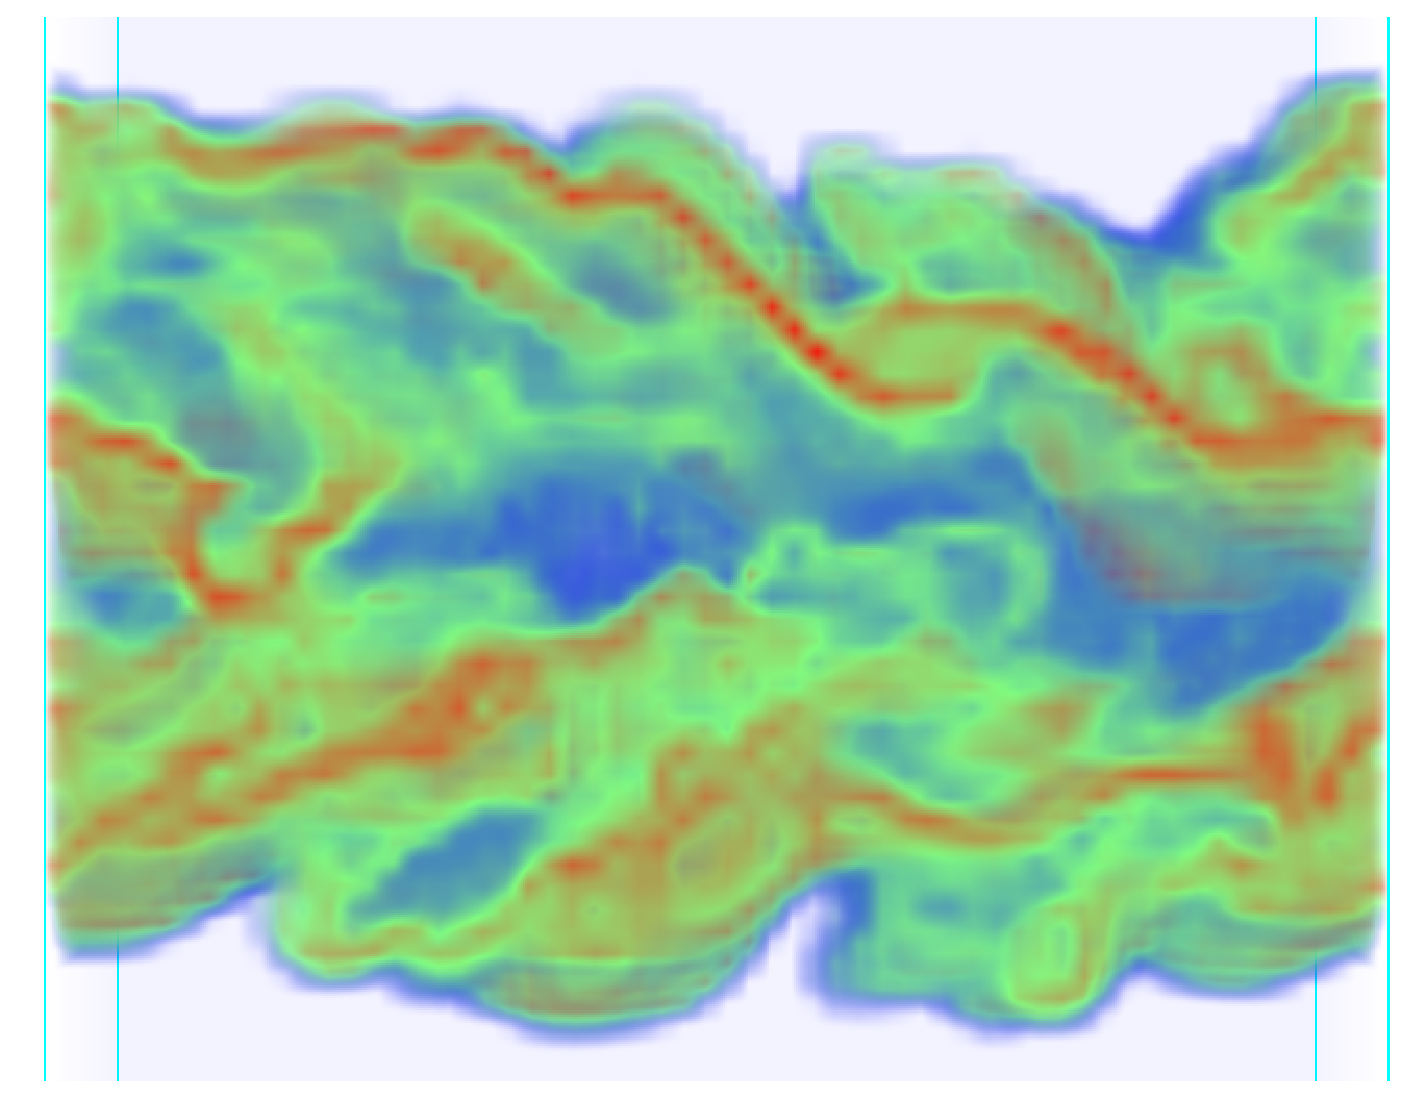
\includegraphics[width = 0.3\linewidth, keepaspectratio = true]{images/eps/mixfrac_entropy.eps}
%	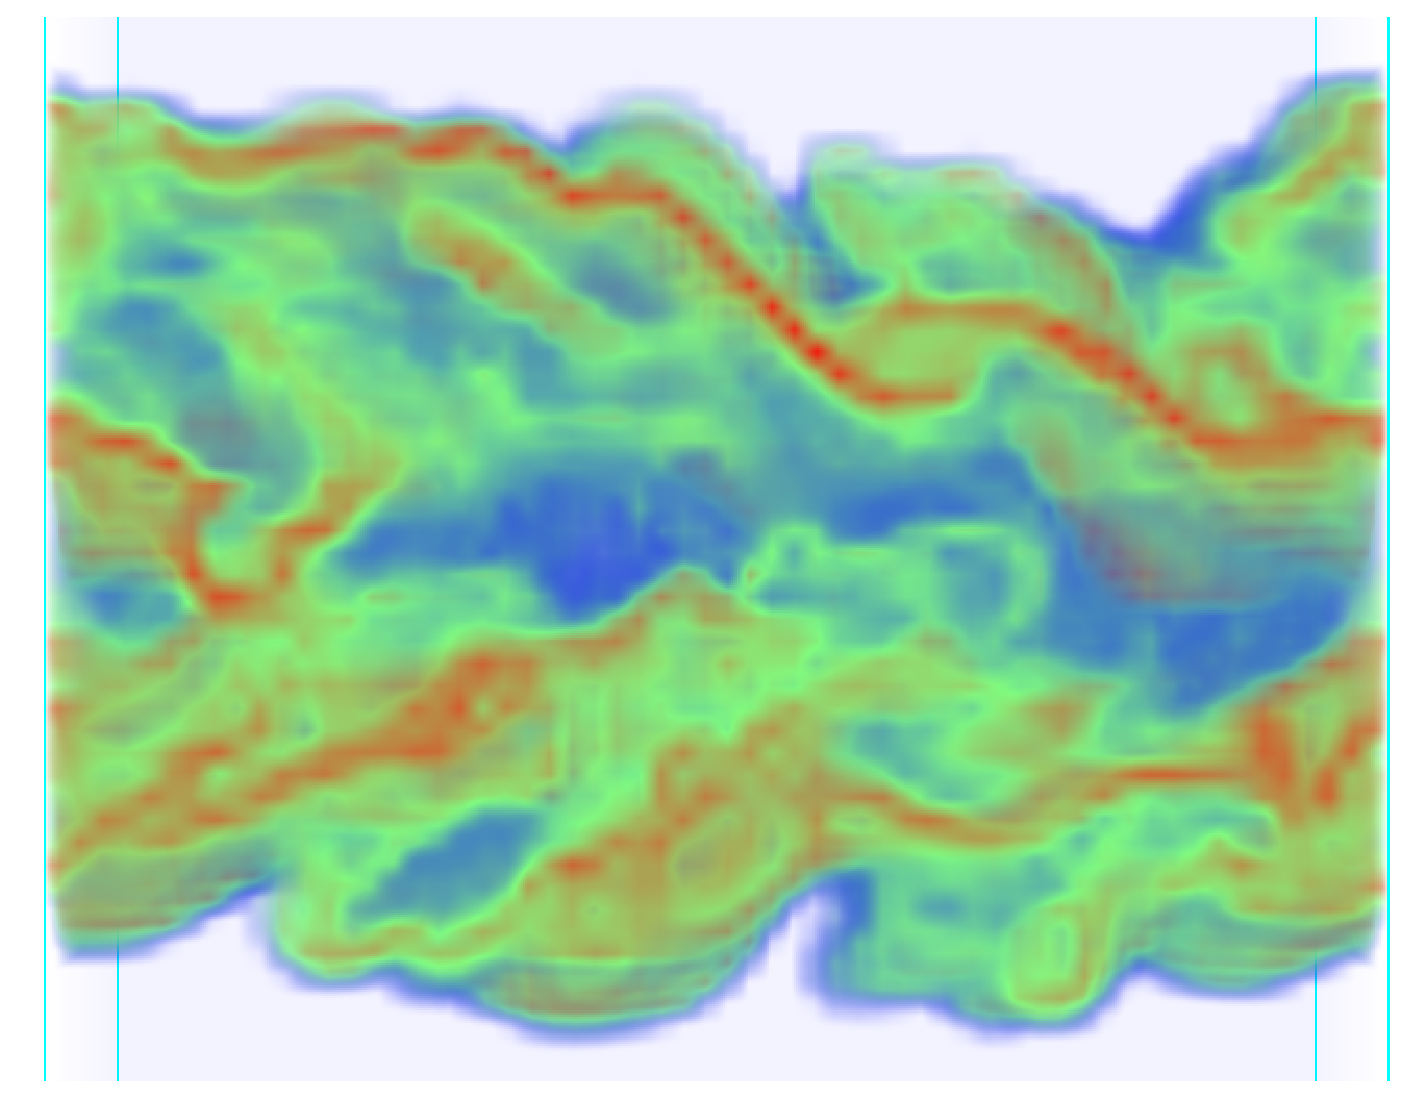
\includegraphics[width = 0.3\linewidth, keepaspectratio = true]{images/eps/mixfrac_entropy.eps}
%	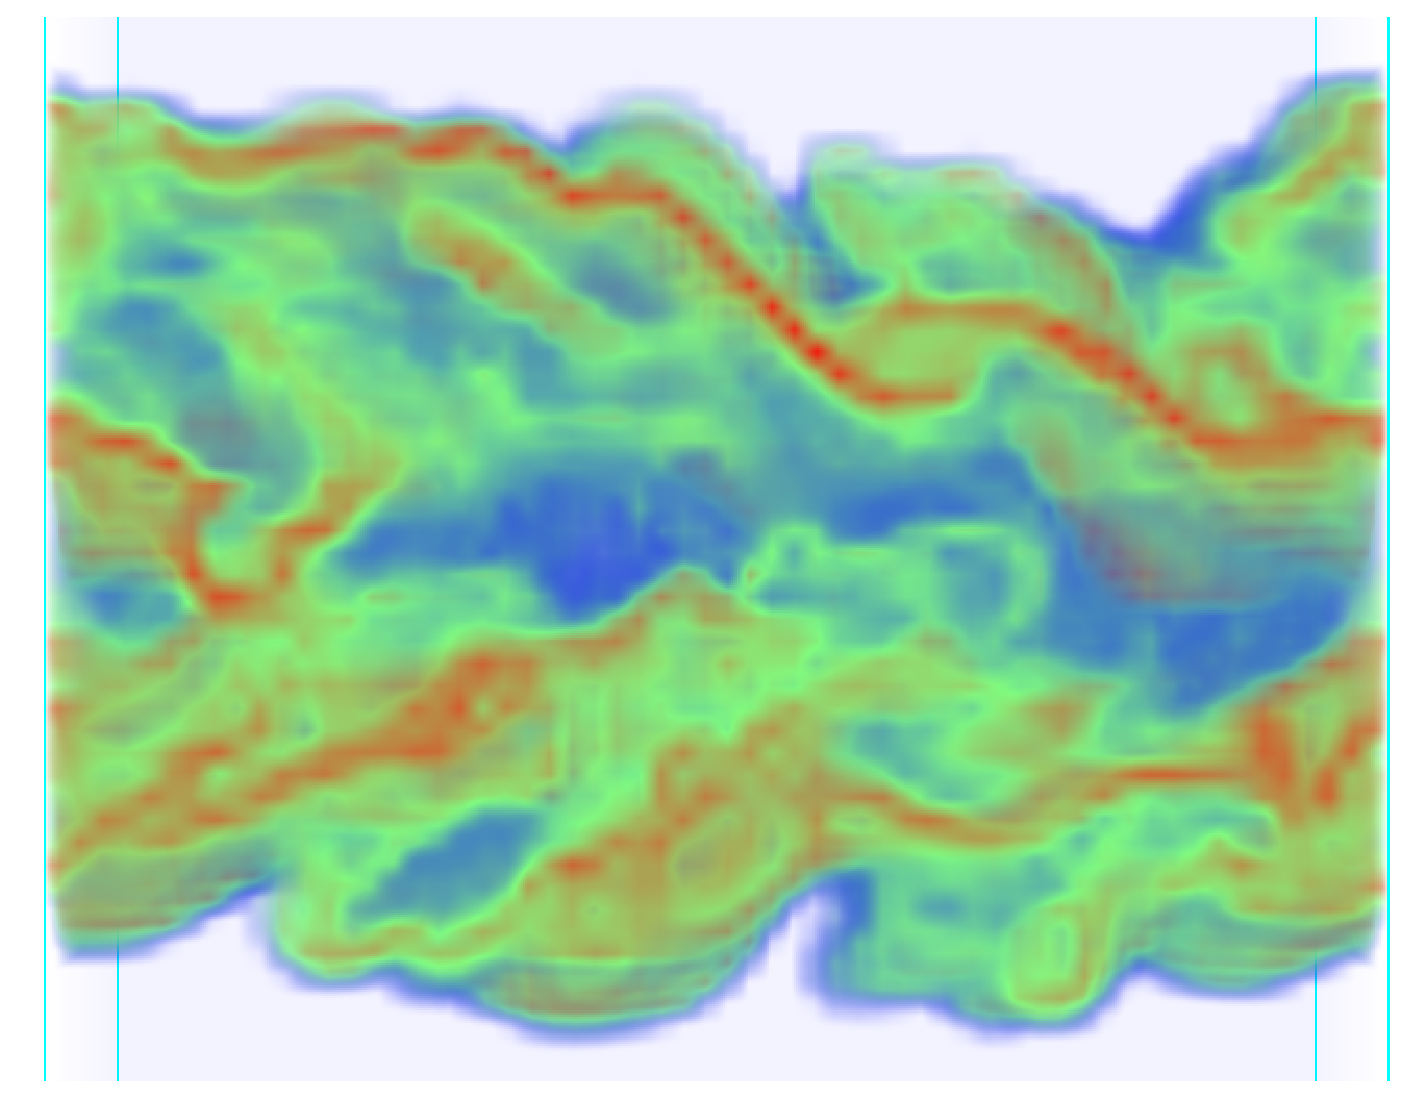
\includegraphics[width = 0.3\linewidth, keepaspectratio = true]{images/eps/mixfrac_entropy.eps}
%	\caption{Pointwise entropy field for different neighborhood sizes. {\bf *** Middle and right image will change ***}}	
%	\label{fig:localstat}
%	%\vspace{0.3cm}
%%\end{figure}
\begin{figure}[tb]
		\centering
		%\subfloat[Distribution based fuzzy isosurface computation for arbitrary resolutions from Isabel Pressure field. {\bf Left.} True isosurfaces. {\bf Middle Column} Volume rendering of likelihood field for block size 4. {\bf Right column} Likelihood field for block size 12.]
		%{\label{fig:fuzzysurface_isabel}
			\includegraphics[width = 0.64\linewidth, keepaspectratio = true]{images/eps/testcase_isabel_1.eps}
		%}
		\caption{Block distribution-based fuzzy isosurface computation for arbitrary levels of detail from Isabel Pressure field. {\bf Top.} True isosurfaces. {\bf Middle.} Likelihood field for -500 Pa. {\bf Bottom.} Likelihood fields for +100 Pa.}	
		\label{fig:fuzzysurface_isabel}
		\vspace{-0.1in}
\end{figure}		
%%%%%%%%%%%%%%%%%%%
%% Diagram ends
%%%%%%%%%%%%%%%%%%%

%We have employed our technique to compute such fields while varying the block size over a range. Figure~\ref{fig:localstat_plot} compares our method's performance against the raw data access method. Clearly, our method's does not depend on the neighborhood size used, while the raw data access method does. 
%%
%%
\subsection{Feature Detection with Fuzzy Isosurfaces}
\label{sec:application_1}
%%
%%
%%%%%%%%%%%%%%%%%%%
%% Diagram begins
%%%%%%%%%%%%%%%%%%%
%\begin{figure*}[tb]
%	\begin{minipage}{\linewidth}
%		\centering
%		\subfloat[Distribution based fuzzy isosurface computation for arbitrary resolutions from Isabel Pressure field. {\bf Left.} True isosurfaces. {\bf Middle Column} Volume rendering of likelihood field for block size 4. {\bf Right column} Likelihood field for block size 12.]
%		{\label{fig:fuzzysurface_isabel}
%			\includegraphics[width = 0.32\linewidth, keepaspectratio = true]{images/eps/testcase_isabel_1.eps}
%		}
%		~
%		\subfloat[Distribution-based search for different patterns on Solar Plume dataset (using a $9^3$ local neighborhood). {\bf Top.} A commonly occurring distribution and {\bf Bottom.} a sparsely present distribution used as template.] 	
%		{\label{fig:fuzzysearch_plume}
%			\includegraphics[width = 0.32\linewidth, keepaspectratio = true]{images/eps/similaritysearch_plume.eps}
%		}
%		\subfloat[Distribution-based search for different patterns on Solar Plume dataset (using a $9^3$ local neighborhood). {\bf Top.} A commonly occurring distribution and {\bf Bottom.} a sparsely present distribution used as template.] 	
%		{\label{fig:fuzzysearch_plume}
%			\includegraphics[width = 0.32\linewidth, keepaspectratio = true]{images/eps/similaritysearch_combustion.eps}
%		}
%	\end{minipage}	
%	\\
%	\begin{minipage}{0.38\linewidth}
%		\centering
%				\subfloat[Performance improvement: local statistics computation. {\bf ***Plot spaceholder***}]	
%		{\label{fig:localstat_plot}
%			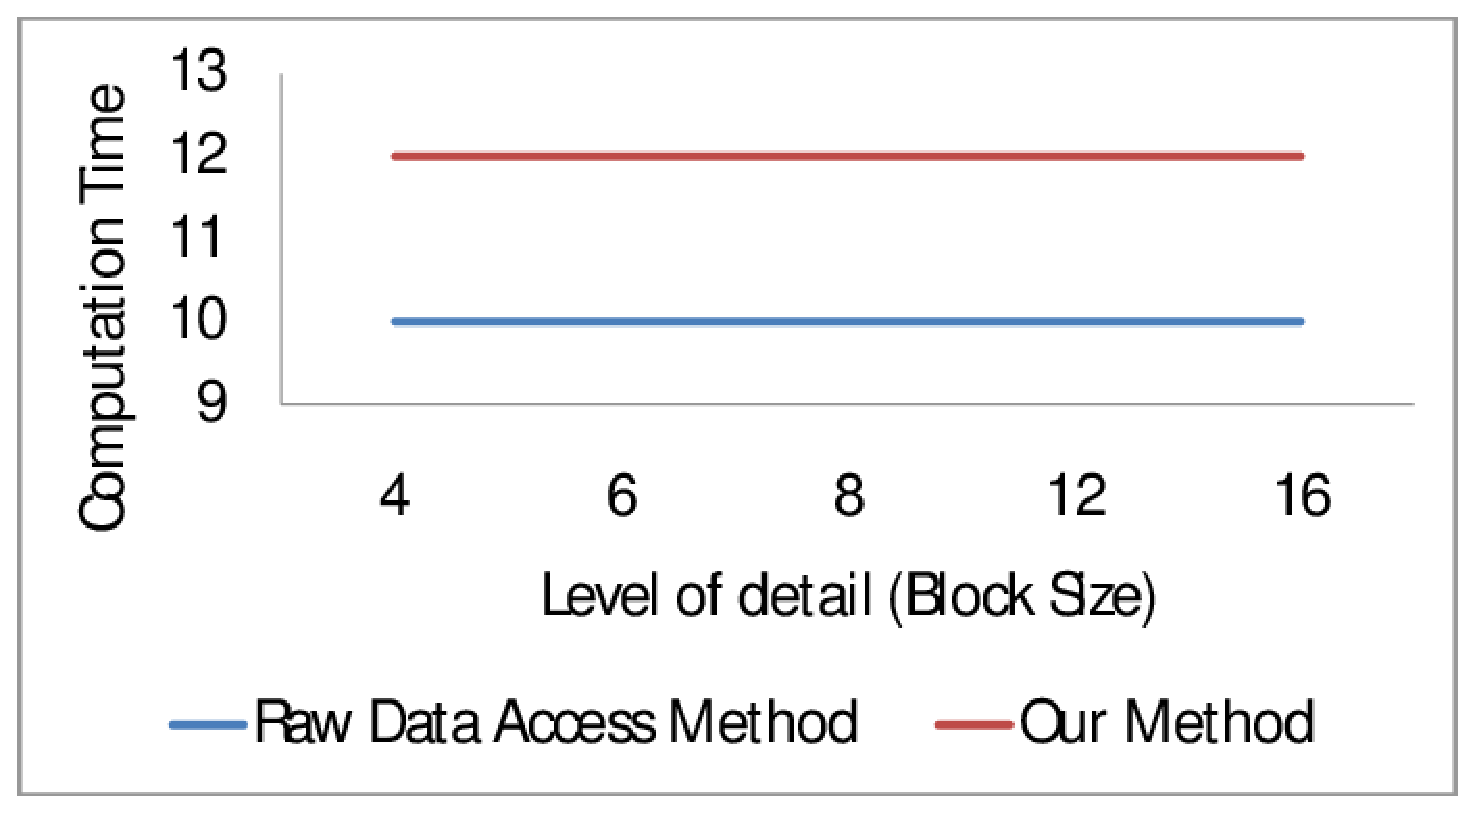
\includegraphics[width = 0.3\linewidth, keepaspectratio = true]{images/eps/plot1.eps}
%		}		
%		~
%		\subfloat[Performance improvement: local statistics computation. {\bf ***Plot spaceholder***}]	
%		{\label{fig:localstat_plot}
%			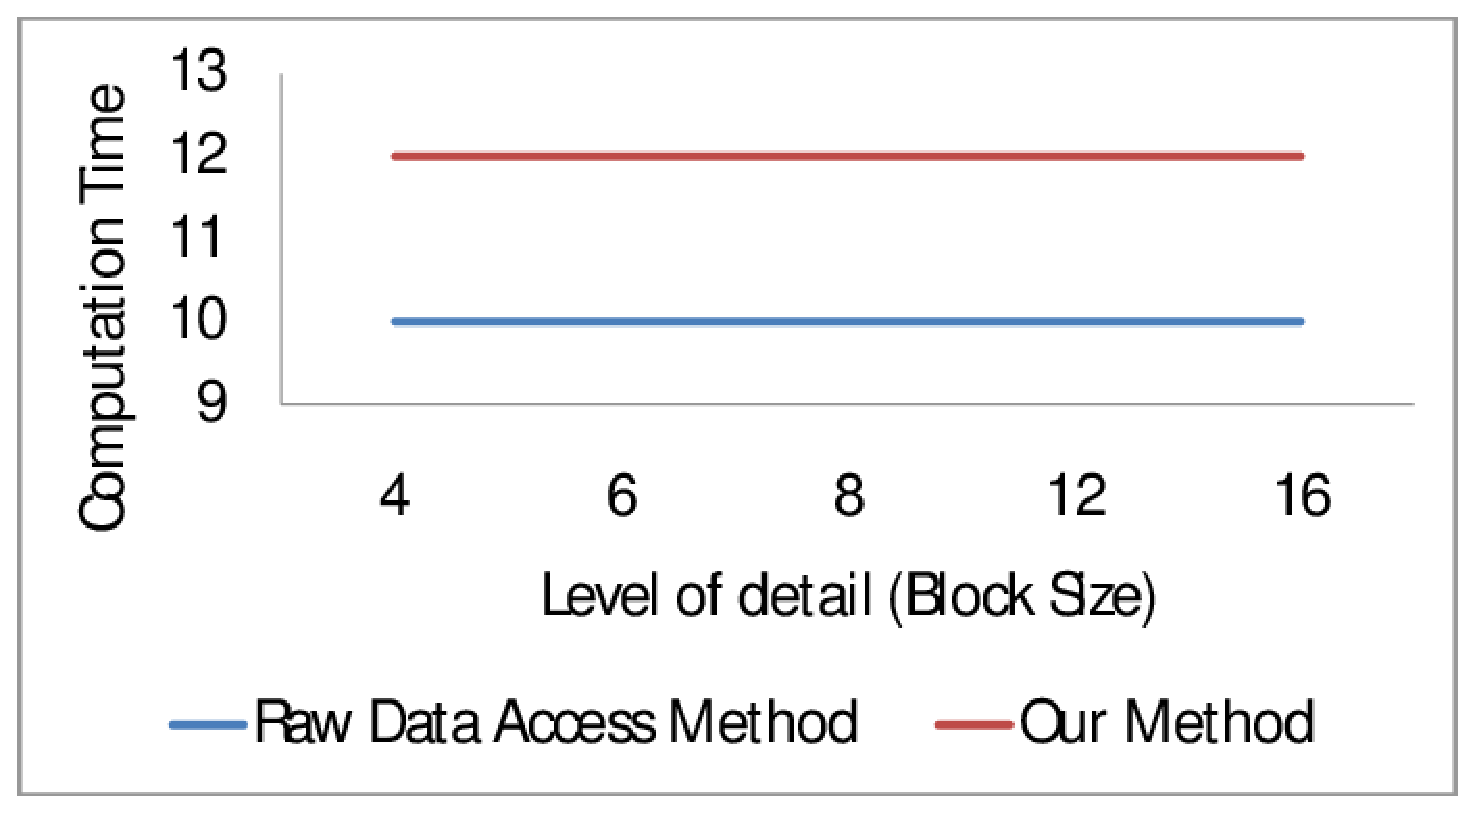
\includegraphics[width = 0.3\linewidth, keepaspectratio = true]{images/eps/plot1.eps}
%		}		
%		~
%		\subfloat[Performance improvement: Fuzzy isosurface {\bf ***Plot spaceholder***}]	
%		{\label{fig:fuzzyiso_plot}
%			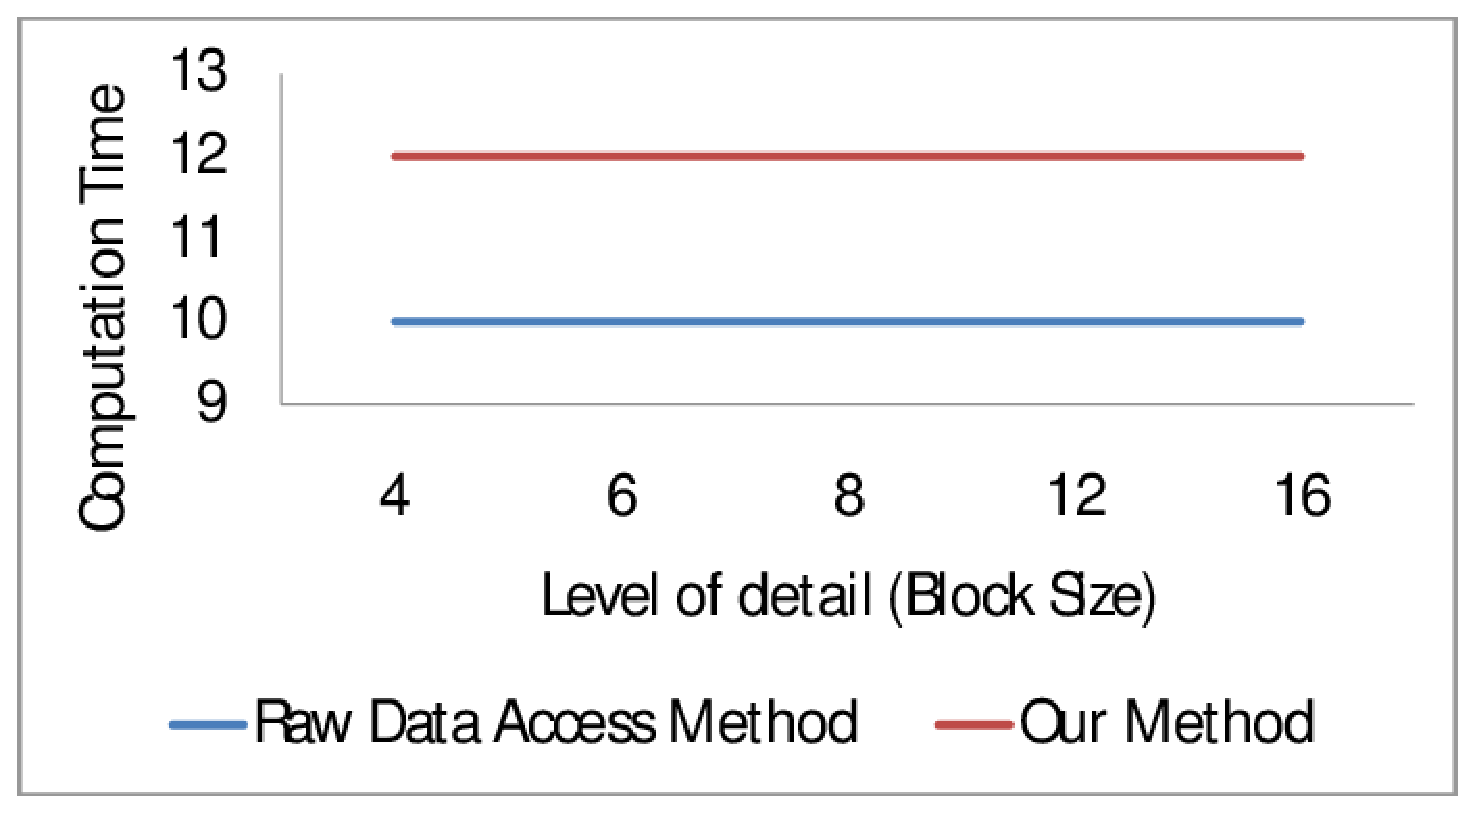
\includegraphics[width = 0.3\linewidth, keepaspectratio = true]{images/eps/plot1.eps}
%		}			
%	\end{minipage}	
%%	~
%%	\begin{minipage}{\linewidth}
%%		\centering
%%		~
%%		~		
%%		\subfloat[Performance improvement: Fuzzy similarity search {\bf ***Plot spaceholder***}]	
%%		{\label{fig:fuzzysearch_plot}
%%			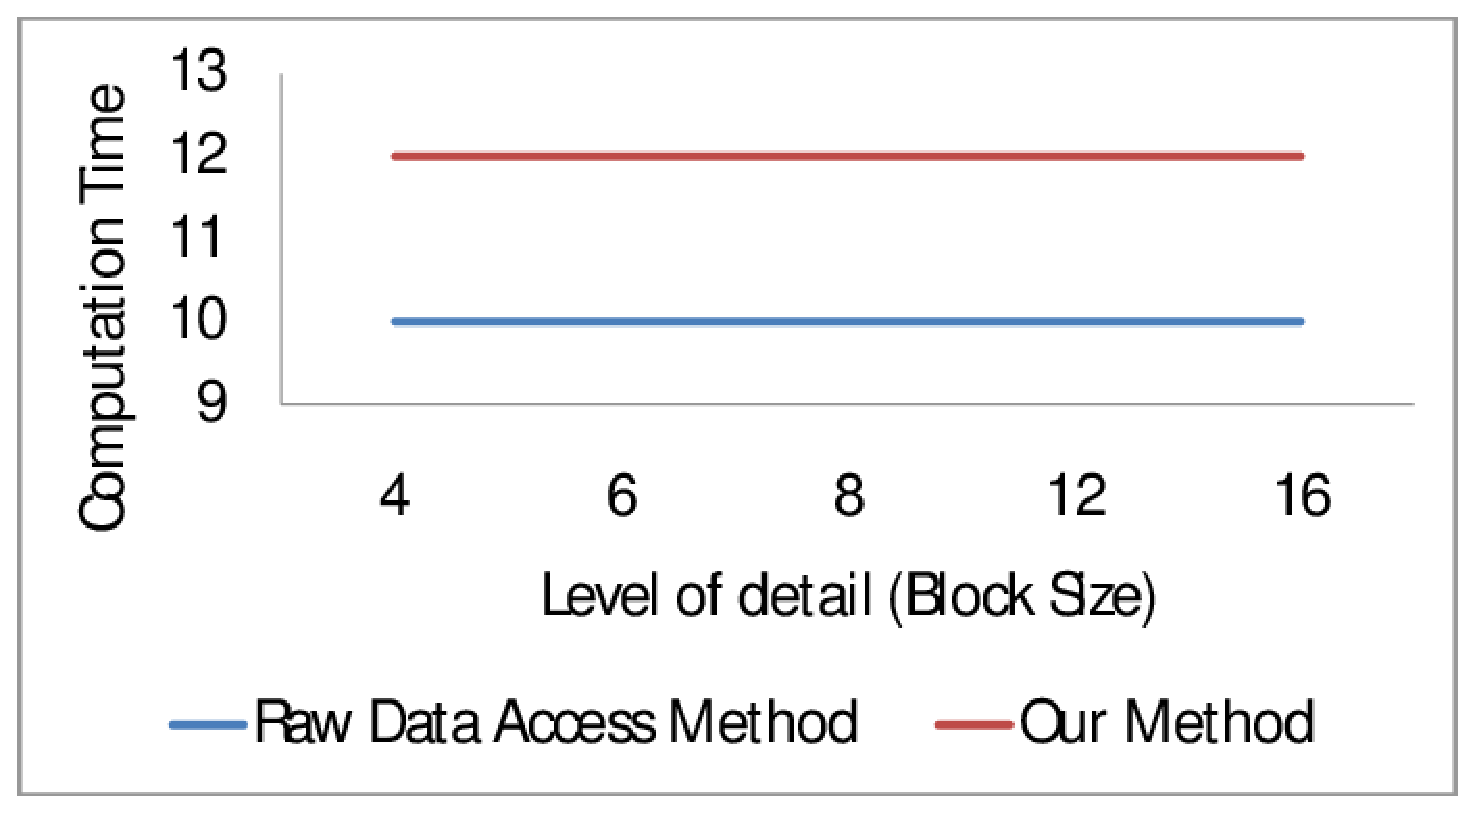
\includegraphics[width = 0.3\linewidth, keepaspectratio = true]{images/eps/plot1.eps}
%%		}		
%%
%%	\end{minipage}	
%
%	\caption{Estimation of various summary statistic using encoded distributions.}
%	
%	\label{fig:applications}	
%\end{figure*}
%%%%%%%%%%%%%%%%%%%
%% Diagram ends
%%%%%%%%%%%%%%%%%%%
%%
We first present an application which runs blockwise distribution queries. Thompson et. al.~\cite{Hixel11} has shown that, in the presence of large-scale data, fuzzy isosurfaces computed from block-level distributions retain the main features present in the original data. When raw data is not available, their technique computes a \emph{likelihood value} for each block for a given isovalue. In the resulting field, zero indicates maximum likelihood of an isovalue being present in a block. However, depending on the required precision and available resources, the user often wants the ability to compute and visualize these likelihood values at different levels of detail. This either requires repeated data access to compute distributions for blocks of varying sizes, or requires storage of pre-computed distributions for a range of block sizes which can easily exceed the data size. Both are impractical for large data. \\
%%
%%%%%%%%%%%%%%%%%%%
%% Diagram begins
%%%%%%%%%%%%%%%%%%%
\begin{figure}[tb]
	\centering
	\subfloat[Distribution-based search on Solar Plume.] 	
	{\label{fig:fuzzysearch_plume}
	\includegraphics[width = 0.7\linewidth, keepaspectratio = true]{images/eps/similaritysearch_plume.eps}}\\
	\subfloat[Distribution-based search on Combustion.] 	
	{\label{fig:fuzzysearch_combustion}
	\includegraphics[width = 0.7\linewidth, keepaspectratio = true]{images/eps/similaritysearch_combustion.eps}}
	\caption{ (a) Distribution-based search for different patterns on Solar Plume dataset (using a $9^3$ local neighborhood). A commonly occurring distribution {\bf (top)}, and a sparsely present distribution {\bf (bottom)} used as template. (b) Distribution-based search for locations with stoichiometric mixture rate of 0.42 on time step 118 of combustion dataset (using a $7^3$ local neighborhood).}
	\label{fig:fuzzysearch}	
	\vspace{-0.1in}
\end{figure}	
%%%%%%%%%%%%%%%%%%%
%% Diagram ends
%%%%%%%%%%%%%%%%%%%

In this situation, our method can fast retrieve the block distributions for any level of detail on demand, without touching the raw data and having to store a large number of distributions. For example, at block size 32, our method finishes a set of 200 block-based queries in 0.11 seconds while the raw data access method takes 2.62 seconds (detailed performance study is in Section~\ref{subsec:analysis_encoding_space}). 

We have shown one example using the pressure field of hurricane Isabel dataset. According to previous research~\cite{qdv11}, pressure values less than -350 Pa correspond to the hurricane eye. The top image in Figure~\ref{fig:fuzzysurface_isabel} shows the  true isosurface for isovalue -500 Pa, (blue surface), which surrounds the hurricane eye, and the isosurface for +100 Pa (orange surface), which spans a large area outside the eye. The middle row contains the likelihood field for isovalue -500 Pa computed from block sizes 4 and 12. The bottom row shows the likelihood fields for +100 Pa for blocks of size 4 and 12. The importance of using different block sizes becomes apparent from the images. For isovalue -500 Pa, having the ability to use higher level of detail is necessary, since it indicates a localized feature with a distinct shape. On the other hand, a bigger block size may be sufficient for understanding isovalue +100 Pa, which does not represent or contain a fine feature. 
%%
%%
\subsection{Distribution-based Similarity Search}
\label{sec:application_2}
%%
%%
The second application is an example of pointwise range distribution query. When the user does not know the exact isovalue to look for, it is more convenient to place the query in the form of a distribution, a Gaussian kernel centering at the best estimated isovalue or a Gaussian mixture for example. If a feature is characterized by a particular type of distribution, that also prompts the user to search for that type of distribution in the data. In this context, Johnson and Huang~\cite{johnson09} has proposed to compute a \emph{fuzzy similarity score} which indicates the similarity between the user-input distribution and a local neighborhood based distribution at each voxel. The resulting similarity field has a score range from 0 to 1, 1 indicating the best match. However, whenever the query changes or the neighborhood size to be used for search changes, this method has to re-compute the distributions at each voxel. Doing this by accessing the raw data becomes very slow since it involves multiple accesses to the every data point. For example, our method computes pointwise distributions at every 4th point (based on a $32^3$ local neighborhood, query set contains total 48.8K points) of \emph{mixfrac} variable of combustion data in 6.15 seconds, while the raw data access method takes 186.65 seconds. 

Figure~\ref{fig:fuzzysearch_plume} shows two examples of distribution based search on Solar Plume. The query for the top image (distribution shown in inset) is a more common one, so most voxels of the resulting field have higher similarity score (red or orange) and only a few regions are dissimilar to the query (shown in blue). On the contrary, the query distribution for the bottom image is a Gaussian mixture where both Gaussians are centered at less probable values. Hence, most of the voxels in the similarity field are 0 or close to 0 (shown in blue). We have modulated the opacity to highlight the two small regions corresponding to the two Gaussian peaks in the query. Figure~\ref{fig:fuzzysearch_combustion} shows a distribution query on mixture fraction variable of Combustion data. We have used a Gaussian distribution centered at 0.42 as the query. The high similarity zones in the search result (red, right image) correspond well to the flame extinction zones (value $\sim$0.42) in the raw data (red, left image).



\section{Quantitative Analysis}
\label{sec:analysis}
%%
%%
In this section, we analyze how we have achieved the main goal of our framework -- reducing storage cost and query workload using transformed distribution data. We have also studied performance of various stages of our framework, and compared our technique with alternate approaches.

\paragraph*{Datasets:} Table~\ref{tbl:datasets} lists the sizes of the datasets used in our experiments. It also presents the size of the integral distribution volume to highlight the huge storage cost associated with it. Loading the entire IDV to memory is not permissible in most cases.
%%
%%%%%%%%%%%%%%%%%%%%%%%%%%%%%%%%%%%%%%%%%
%% Table begins
%%%%%%%%%%%%%%%%%%%%%%%%%%%%%%%%%%%%%%%%%
\begin{table}[!htb]
	\centering	
	\renewcommand{\tabcolsep}{0.09cm}
	\begin{tabular}{|c|c|c|c|}
		\hline
		{\small Dataset} & {\small Size} & {\small Number} & {\small Integral Distribution}\\		
		{\small } & {\small } & {\small of bins} & {\small Volume Size (GB)}\\		
		\hline			
		{\small Plume} & {\small 126x126x512} & {\small 64} & {\small 3.29}\\
		{\small Isabel} & {\small 250x250x50} & {\small 64} & {\small 1.49}\\
		{\small Combustion} & {\small 240x360x60} & {\small 64} & {\small 2.47}\\
		\hline		
	\end{tabular}
	\vspace{-0.3cm}	
	\caption{\label{tbl:datasets} Size of datasets used and the storage cost of corresponding IDVs.}
\end{table}
%%%%%%%%%%%%%%%%%%%%%%%%%%%%%%%%%%%%%%%%%%%%%%%%%%%
%% Table ends
%%%%%%%%%%%%%%%%%%%%%%%%%%%%%%%%%%%%%%%%%%%%%%%%%%%	

For all experiments on all datasets, we have partitioned the data into 1024 blocks and performed both the pre-processing and the query in parallel. Even though our primary focus is not on designing a sophisticated parallel algorithm, we have worked with partitioned data to emphasize the need for our method on large distributed data.

\paragraph*{Alternate Methods:} In terms of storing integral distributions, we have compared against the most straightforward alternative: directly compressing IDV using any off-the-shelf compression scheme. The second alternative is to run the proposed indexing algorithm directly on the IDV, bypassing the decomposition into power-of-two length sub-ranges, and to compress the indexing output. This alternative is presented to justify the importance of the decomposition step in our framework. Finally, we present results from our method which performs decomposition into sub-ranges, then indexing of sub-ranges and finally, compression. 

The third stage -- compression of indexing results -- works with any compression scheme. We have shown results using standard implementations of LZ (Lempel-Ziv)~\cite{lz77} and bzip2 algorithms. Our work does not recommend any particular compression algorithm. Our objective is to transform IDV, which is originally not easy to compress, to an easily compressible form.

In terms of query performance, we have compared against \emph{raw data access} method. Raw data access is a simple load-and-filter approach where, given a range query, each data block that falls within the query is loaded from disk and scanned to compute the partial or full distribution. All these partial distributions are then combined to obtain the final query result. 
%%
%%
\subsection{Space Saving}
\label{sec:analysis_encoding_space}
%%
%%
The primary benefit of our method is that it enables use of integral distributions by reducing its storage cost. When the data is partitioned into $p$ blocks, the \emph{space saving} due to encoding is measured by $\big ( 1 - \frac{\sum_{i=1}^{p} \text{Size of codebook}}{\text{Size of IDV}} \big )$, represented as a percentage. Size of the codebook (for each data block) is the sum of the following: $<$index, transformation$>$ pairs for each sub-range histogram (one integer plus one boolean per histogram), and the compressed residual frequencies after indexing. The utilized templates also need to be stored once for all blocks. To give an idea, the number of templates to be stored for Plume, Isabel and Combustion data are only 403, 249 and 269.

Figure~\ref{fig:spacesaving} presents the space saving obtained by our method and compares it against two other techniques. Space saving for all three methods are measured with respect to the storage cost of the actual IDV. For each group, the leftmost bar indicates the space saving achieved when the IDV is directly compressed using a lossless compression technique such as LZ and bzip2. The middle bar in each group is the result of skipping the sub-range transformation and directly running our indexing algorithm. However, the results indicate that the original distributions from IDV do not lend themselves very well to an indexing algorithm. This justifies the necessity of the transformation into sub-ranges. Finally, we show that our method, combining transformation, indexing and compression, leads to very high space saving (the rightmost bars in each group). 
%%
%%
%%%%%%%%%%%%%%%%%%%
%% Diagram begins
%%%%%%%%%%%%%%%%%%%
\begin{figure}[tb]
\centering
	\subfloat[Compression method used on indexing result: LZ]{\label{fig:spacesaving_lz}
	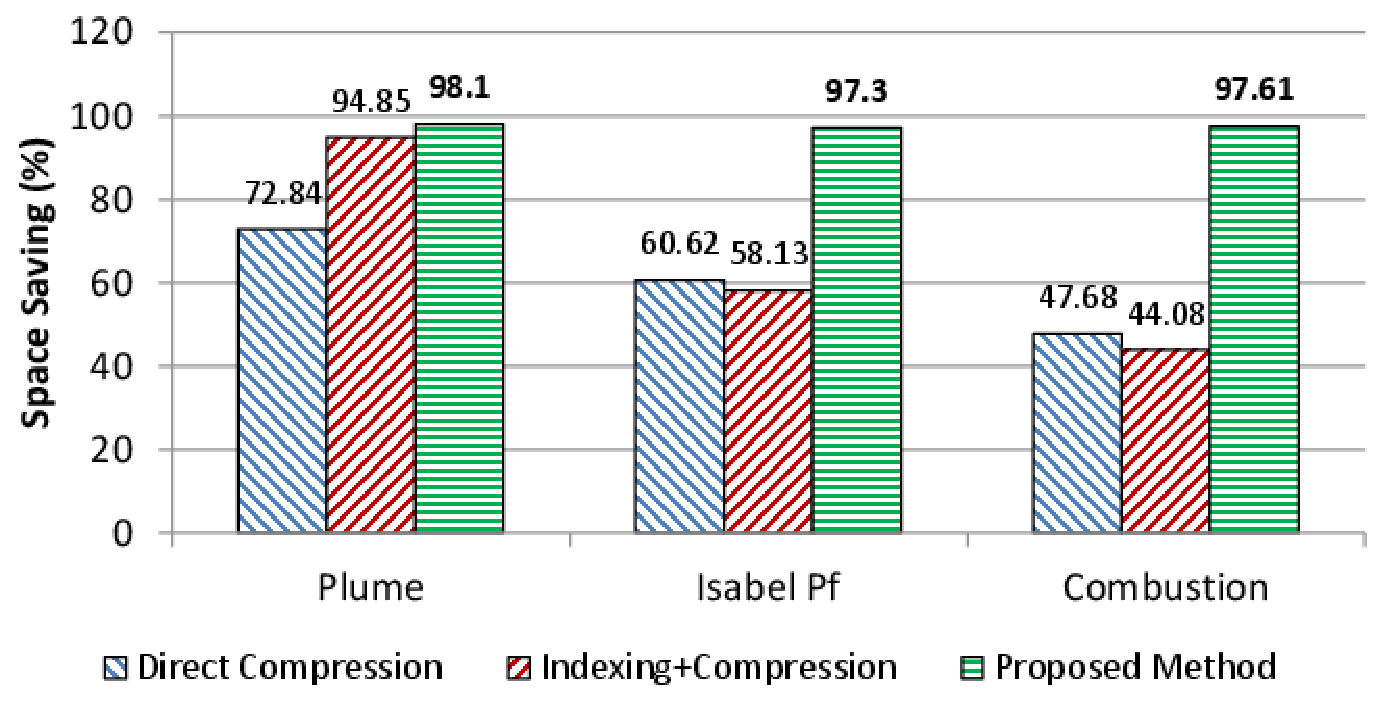
\includegraphics[width = 0.78\linewidth, keepaspectratio = true]{images/eps/spacesaving_lz.eps}}\\
	~
	\subfloat[Compression method used  on indexing result: bzip2]{\label{fig:spacesaving_bz2}
	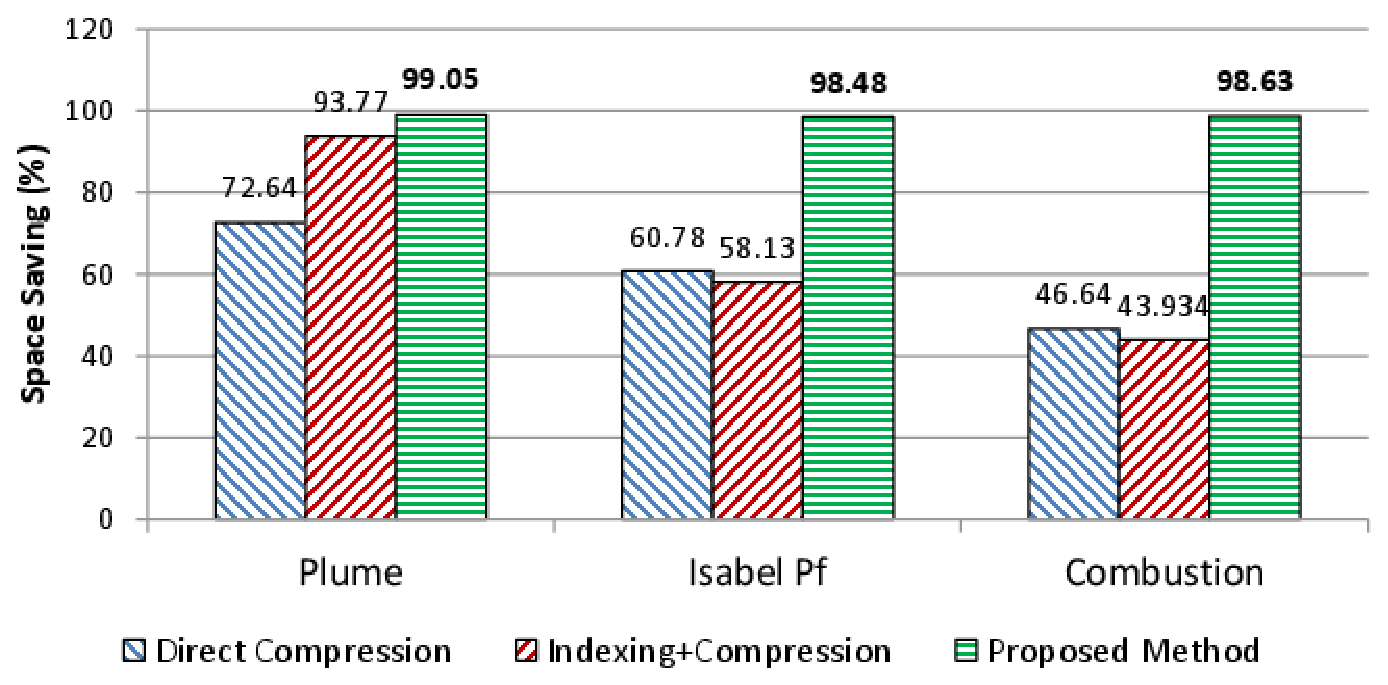
\includegraphics[width = 0.78\linewidth, keepaspectratio = true]{images/eps/spacesaving_bz2.eps}}
	\caption{Space saving achieved by our method (right bars in each group) and two other methods: direct compression of IDV (left bars) and compression after direct indexing of IDV (middle bars).}	
	\label{fig:spacesaving}
\end{figure}
%%%%%%%%%%%%%%%%%%%
%% Diagram ends
%%%%%%%%%%%%%%%%
%%
%%%%%%%%%%%%%%%%%%%%%%%%%%%%%%%%%%%%%%%%%%
%%% Table begins
%%%%%%%%%%%%%%%%%%%%%%%%%%%%%%%%%%%%%%%%%%
%\begin{table}[tb]
%	\centering	
%	\renewcommand{\tabcolsep}{0.09cm}
%	\begin{tabular}{|c|c|c|c|c|}
%		\hline
%		{\small Dataset} & {\small Compression} & \multicolumn{3}{|c|}{\small Space Saving}\\		
%		{\small } & {\small Technique} & \multicolumn{3}{|c|}{\small (\%)}\\		
%		\hline
%		{\small } & {\small } & {\small Direct} & {\small Indexing+} & {\small {\bf Proposed}}\\
%		{\small } & {\small } & {\small Compression}& {\small Compression} & {\small {\bf Method}}\\
%		\hline
%		%{\small } & {\small RLE} & {\small 5.84} & {\small 5.84} & {\small 69.14} & {\small {\bf 91.45}}\\	%5.84301
%		{\small Plume} & {\small LZ} & {\small 72.84} & {\small 94.85} & {\small {\bf 99.14}}\\	%94.85
%		{\small } & {\small BZ2} & {\small 72.64} & {\small 93.77} & {\small {\bf 99.5}}\\		%93.77
%		\hline
%		%{\small } & {\small RLE} & {\small 5.84} & {\small 5.84} & {\small 69.14} & {\small {\bf 91.45}}\\	%5.84301
%		{\small Isabel} & {\small LZ} & {\small 60.62} & {\small 58.13} & {\small {\bf 97.30}}\\	%94.85
%		{\small } & {\small BZ2} & {\small 60.78} & {\small 58.13} & {\small {\bf 98.48}}\\		%93.77
%		\hline
%		%{\small } & {\small RLE} & {\small 5.84} & {\small 5.84} & {\small 69.14} & {\small {\bf 91.45}}\\	%5.84301
%		{\small Combustion} & {\small LZ} & {\small 47.68} & {\small 44.08} & {\small {\bf 97.61}}\\	%94.85
%		{\small } & {\small BZ2} & {\small 46.64} & {\small 43.934} & {\small {\bf 99.5}}\\		%93.77
%		\hline		
%	\end{tabular}
%	\caption{\label{tbl:storagecomp} Storage Reduction by Proposed Technique. Pre-processing is done on 8 processors in parallel. {\bf Isabel and combustion numbers are running}}
%\end{table}
%%%%%%%%%%%%%%%%%%%%%%%%%%%%%%%%%%%%%%%%%%%%%%%%%%%%
%%% Table ends
%%%%%%%%%%%%%%%%%%%%%%%%%%%%%%%%%%%%%%%%%%%%%%%%%%%%	
%%
%%
%%
\subsection{Faster Query Response}
\label{subsec:analysis_encoding_space}
%%
%%
According to our hypothesis, the performance of query in our method should not depend on query size, as we use integral histogram. We have tested this hypothesis by varying the query size from $16^3$ to $48^3$. For each query size, we have used a set of 2000 queries coming from different locations of the data. As shown in Figure~\ref{fig:blockqueryresponse_1}, our method is much faster than the raw data access method for each dataset and across all query sizes. The total time taken by our method always remains less than 0.1 second, while the time taken by raw data access method varies linearly with query size. More importantly, Figure~\ref{fig:blockqueryresponse_2} shows that the speed-up obtained by our method compared to accessing raw data keeps increasing with the query size. This indicates that our method handles larger queries more efficiently, and hence, suits larger datasets.

The above experiment corresponds to the pointwise and blockwise query types. We have also tested the performance of queries whose sizes vary randomly. Each query in the set is a 3D sub-domain centered at the center of the full spatial domain. This allows the query size to vary to the maximum possible extent along each dimension. Figure~\ref{fig:randomqueryresponse} shows that our method provides faster query response (compared to raw data access) for random query as well. The achieved speed-up in total response time for 2000 queries on Plume, Isabel pressure and Combustion dataset are 95.8x, 98.95x and 267x respectively. 

For all our experiments, each dataset is partitioned into 1024 blocks, and the query is computed on 8 processors in parallel. The performance numbers are based on an Intel(R) Core(TM) i7-2600 3.4GHz quad-core processor with 16GB memory.

%Depending on the disk space available, the pre-processed results can be stored as it is, or compressed using some technique. If the data needs to be decompressed during query phase, some computation overhead is added. Hence, for each method, the overhead associated with different compression techniques has been compared.
%%
%%
%%%%%%%%%%%%%%%%%%%
%% Diagram begins
%%%%%%%%%%%%%%%%%%%
\begin{figure}[tb]
\centering	
	\subfloat[Query response time of our method across different query sizes]{\label{fig:blockqueryresponse_1}
	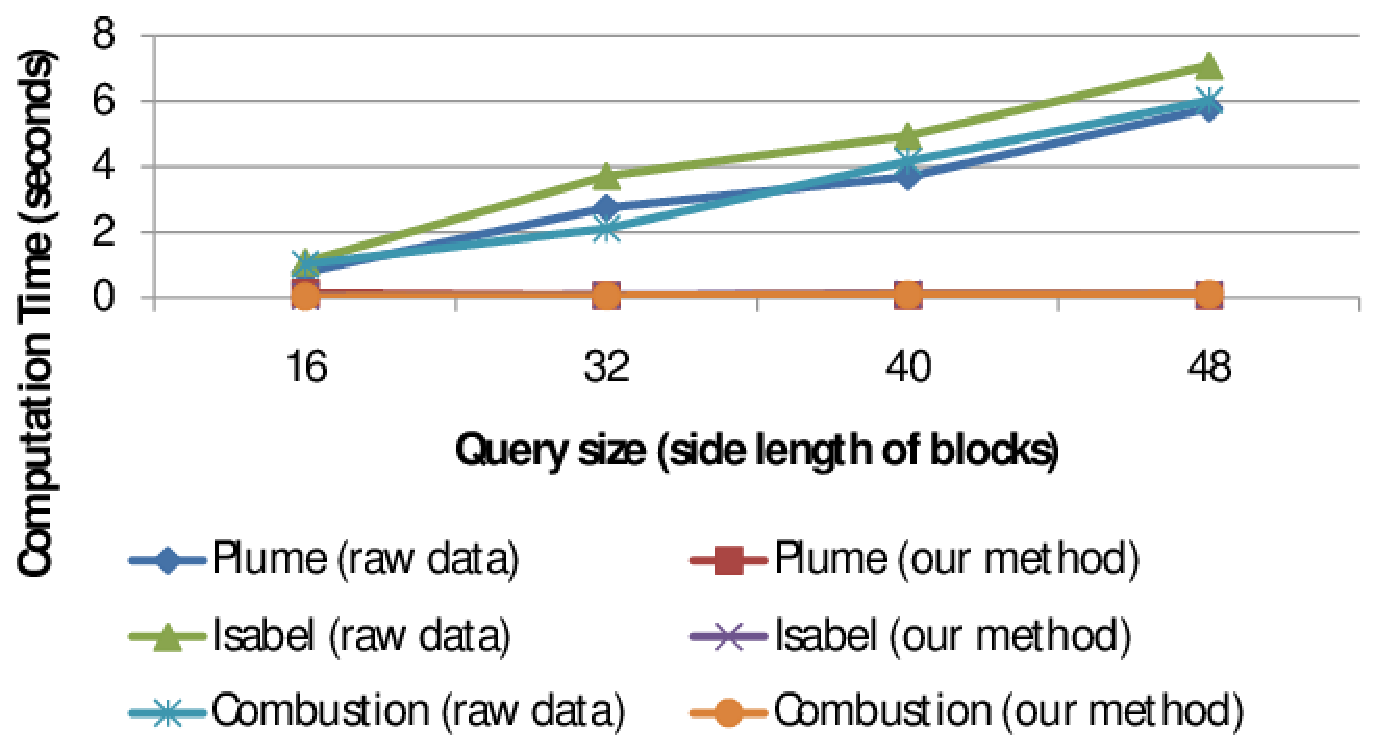
\includegraphics[width = 0.78\linewidth, keepaspectratio = true]{images/eps/block_query_abs.eps}}\\
	\subfloat[Speed-up achieved by our method across different query sizes]{\label{fig:blockqueryresponse_2}
	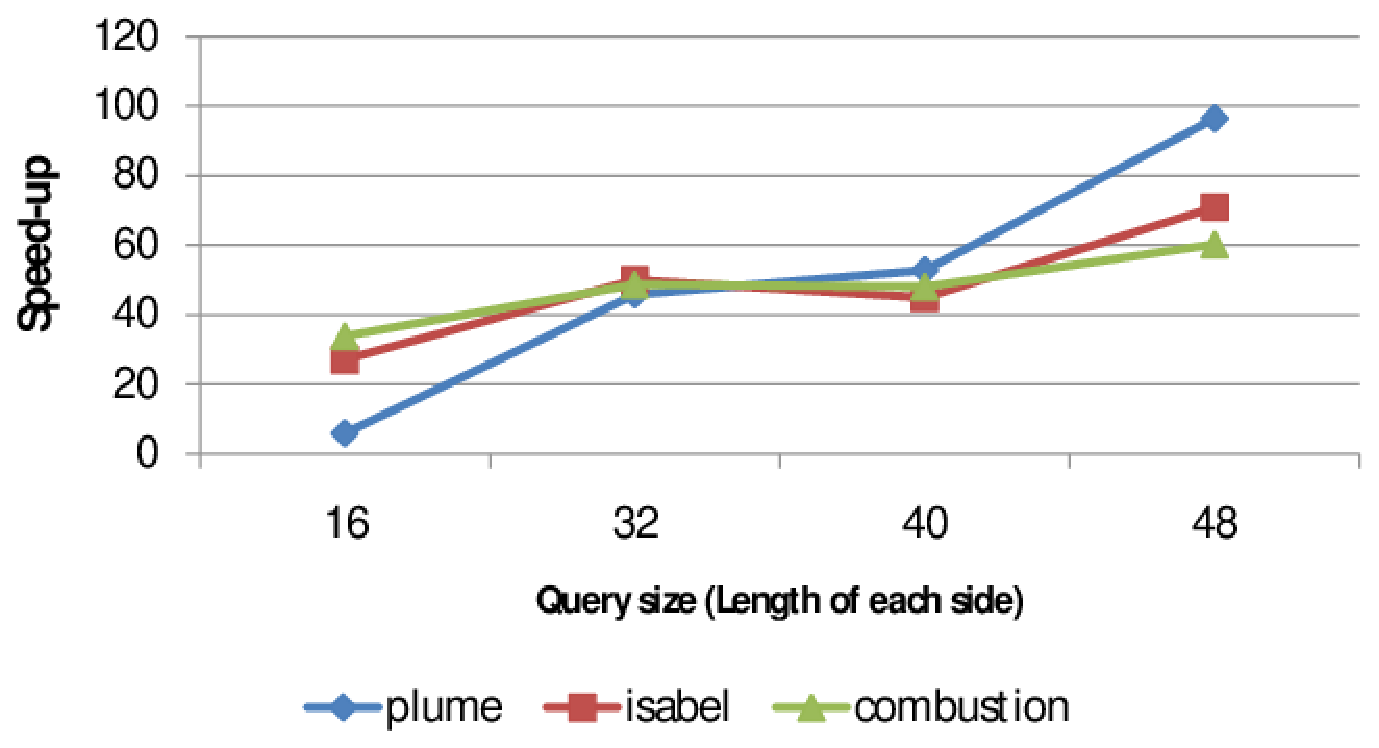
\includegraphics[width = 0.78\linewidth, keepaspectratio = true]{images/eps/block_query_rel.eps}}\\
	\subfloat[Query response time of our method for queries of mixed sizes. Average side length of each query is 101.3 for Plume, 72.66 for Isabel, and 86.84 for Combustion.]{\label{fig:randomqueryresponse}
	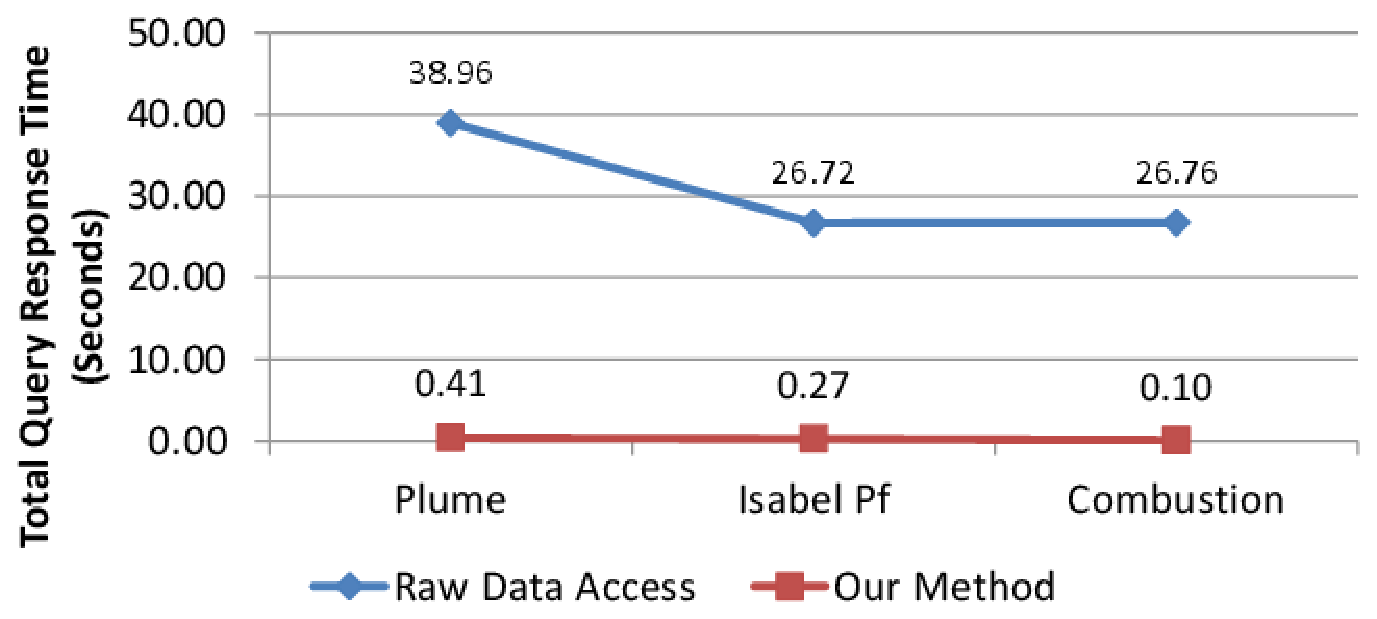
\includegraphics[width = 0.78\linewidth, keepaspectratio = true]{images/eps/random_query.eps}}
	\caption{Performance analysis of query response for different query sizes and different datasets.}	
	\label{fig:queryresponse}
	\vspace{-0.2in}
\end{figure}
%%%%%%%%%%%%%%%%%%%
%% Diagram ends
%%%%%%%%%%%%%%%%
%%
%%
%%%%%%%%%%%%%%%%%%%%%%%%%%%%%%%%%%%%%%%%%%
%%% Table begins
%%%%%%%%%%%%%%%%%%%%%%%%%%%%%%%%%%%%%%%%%%
%\begin{table}[tb]
%	\centering	
%	\renewcommand{\tabcolsep}{0.09cm}
%	\begin{tabular}{|c|c|c|c|c|c|c|}
%		\hline
%		{\small Dataset} & {\small De-comp} & \multicolumn{5}{|c|}{\small Total Query Response Time}\\		
%		{\small } & {\small Technique} & \multicolumn{5}{|c|}{\small (seconds)}\\		
%		\hline
%		{\small } & {\small } & {\small Raw Data} & {\small Direct} & {\small Indexing+} & {\small Compression} & {\small {\bf Proposed}}\\
%		{\small } & {\small } & {\small Access}& {\small comp.} & {\small comp.} & {\small of blocks} & {\small {\bf Method}}\\
%		\hline
%		{\small } & {\small None} & {\small 61.35} & {\small 55.97} & {\small 2.81} & {\small 10.15} & {\small {\bf 12.23}}\\	%5.84301
%		{\small Plume} & {\small LZ} & {\small 0} & {\small 0} & {\small 0} & {\small 0} & {\small {\bf 0}}\\	%94.85
%		{\small } & {\small BZ2} & {\small 0} & {\small 0} &  {\small 0} & {\small 0} & {\small {\bf 0}}\\		%93.77
%		\hline
%		%{\small } & {\small RLE} & {\small 5.84} & {\small 5.84} & {\small 69.14} & {\small {\bf 91.45}}\\	%5.84301
%		{\small Isabel} & {\small LZ} & {\small 0} & {\small 0} & {\small 0} & {\small 0} & {\small {\bf 0}}\\	%94.85
%		{\small } & {\small BZ2} & {\small 0} & {\small 0} & {\small 0} & {\small 0} & {\small {\bf 0}}\\		%93.77
%		\hline
%		%{\small } & {\small RLE} & {\small 5.84} & {\small 5.84} & {\small 69.14} & {\small {\bf 91.45}}\\	%5.84301
%		{\small Combustion} & {\small LZ} & {\small 0} & {\small 0} & {\small 0} & {\small 0} & {\small {\bf 0}}\\	%94.85
%		{\small } & {\small BZ2} & {\small 0} & {\small 0} & {\small 0} & {\small 0} & {\small {\bf 0}}\\		%93.77
%		\hline				
%	\end{tabular}
%	\vspace{-0.3cm}	
%	\caption{\label{tbl:query} Improved Query Response Time by proposed technique. {\bf Isabel and combustion numbers are running}}
%\end{table}
%%%%%%%%%%%%%%%%%%%%%%%%%%%%%%%%%%%%%%%%%%
%%% Table ends
%%%%%%%%%%%%%%%%%%%%%%%%%%%%%%%%%%%%%%%%%%
%
%%
\subsection{Performance Study}
\label{sec:analysis_time}
%%
%%
We have parallelized both the pre-processing and the query stages by partitioning the data into blocks and distributing the blocks across many processors. The pre-processing  (decomposition+indexing+compression) stage is easily adaptable to a parallel framework. In a parallel setting, each processor simultaneously computes its own list of templates based on the blocks assigned to it. A global list of templates is then created by accumulating the local lists. The global list is then distributed back to every processor. A global list is used for indexing because even if two blocks are spatially far apart, they may contain similar distributions. After template creation, each data block is decomposed into sub-ranges and then indexed in its own local co-ordinates space. To compensate for this local transformation, the integral distributions (in global coordinates space) for the corner point, three faces and three edges of the preceding blocks are also stored. Table~\ref{tbl:encodingperf} presents the running times of these stages and the time spent to compress the indexing results for different datasets. 
%%
%%%%%%%%%%%%%%%%%%%%%%%%%%%%%%%%%%%%%%%%%%
%%% Table begins
%%%%%%%%%%%%%%%%%%%%%%%%%%%%%%%%%%%%%%%%%%
\begin{table}[tb]
	\centering	
	\renewcommand{\tabcolsep}{0.09cm}
	\begin{tabular}{|c|c|c|c|c|}
		\hline
		{\small Dataset} & {\small Template} & {\small Sub-range} & {\small Compression} & {\small Compression}\\		
		{\small } & {\small Creation} & {\small Decomposition} & {\small (LZ)} & {\small {BZ2}}\\		
		\hline
		{\small Plume} & {\small 0.26} & {\small 0.09} & {\small 77.49} & {\small 256.02}\\
		{\small Isabel} & {\small 0.07} & {\small 0.04} & {\small 188.59} & {\small 194.77}\\
		{\small Combustion} & {\small 0.09} & {\small 0.07} & {\small 173.899} & {\small 204.262}\\
		\hline				
	\end{tabular}
	\caption{\label{tbl:encodingperf} Performance analysis of different stages of pre-processing (run on 8 processors in parallel). All times are in seconds.}
\end{table}
%%%%%%%%%%%%%%%%%%%%%%%%%%%%%%%%%%%%%%%%%%
%%% Table ends
%%%%%%%%%%%%%%%%%%%%%%%%%%%%%%%%%%%%%%%%%%

The main indexing algorithm is computationally expensive since it compares each sub-range against each template. This is why we have tested the scalability of this stage on Surveyor, an IBM BG/P supercomputer at Argonne National Laboratory. Surveyor contains 1024 quad-core nodes, 2TB memory and utilizes the General Parallel File System (GPFS). Figure~\ref{fig:perf_encoding} shows that the indexing performance scales well with number of processors for all three datasets (each partitioned into 1024 blocks).
%%
%%%%%%%%%%%%%%%%%%%%%%%%%%%%%%%%%%%%%%%%%
%% Figure begins
%%%%%%%%%%%%%%%%%%%%%%%%%%%%%%%%%%%%%%%%%
\begin{figure}[!htb]
\centering
	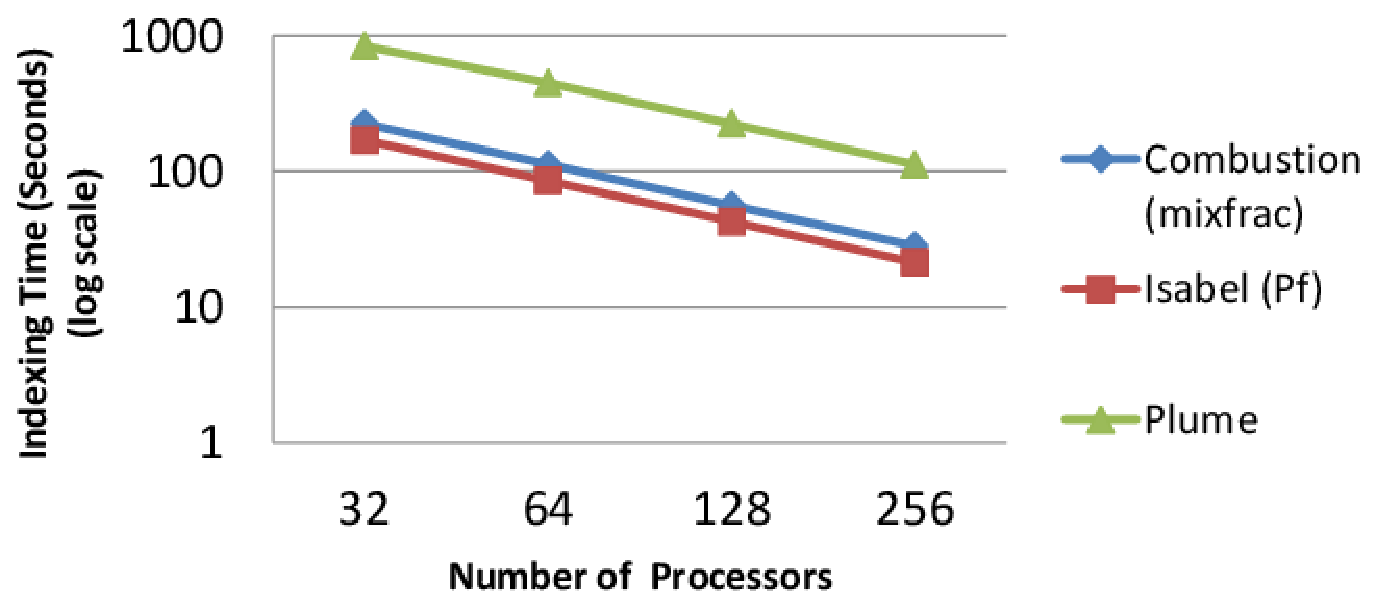
\includegraphics[width = 0.8\linewidth, keepaspectratio = true]{images/eps/perf_encoding.eps}
	\caption{Performance analysis of indexing of power-of-two sub-range distributions from three datasets (each partitioned into 1024 blocks).}	
	\label{fig:perf_encoding}
	\vspace{-0.15in}
\end{figure}
%%%%%%%%%%%%%%%%%%%%%%%%%%%%%%%%%%%%%%%%%%%%%%%%%%%
%% Figure begins
%%%%%%%%%%%%%%%%%%%%%%%%%%%%%%%%%%%%%%%%%%%%%%%%%%%	
%
%%

%\input{sections/timevarying.tex}
\section{Discussion}
\label{sec:discussion}
%%
%%
In essence, we propose transformations to the raw data to make it more compressible. The user should choose the right compression technique depending on whether speed or storage is more critical in the query phase. For example, a method with lower compression rate and faster decompression time (such as LZ) may suit interactive visualization applications, while a slower algorithm producing better compression such as BZ2 is more useful for generating static fields and images from very large data. Figure~\ref{fig:spacesaving_lz} and Fig~\ref{fig:spacesaving_bz2} allow us to compare compression rates of the two techniques we have experimented with. As expected, bzip2 provides slightly better compression than LZ at the cost of performance (Table~\ref{tbl:encodingperf}). The user can increase the compression level of bzip2 (1 used) to save more space at the cost of time.

We have presented query performance without the decompression time. This is because our IDV size is 64 times the data size (64 bins used), and the codebook size (about 1\% of the IDV) is smaller than even the raw data. Hence, under the same available resources, either both raw data and codebook can be loaded uncompressed, or both need to be decompressed. When decompression is needed, only a few locations are to be decompressed and read from the codebook of each block. On the other hand, full data blocks, or significant fractions of them are to be decompressed to access the needed data.

%\paragraph*{Number of Templates:} The template creation technique stands on the assumption
%that a very small number of templates is sufficient due to
%self-similarity present in the data and the distributions. We
%investigate if our template creation strategy produces sufficient
%number of templates. We find that for all the datasets, the encoding
%is performed under the desired threshold only with a fraction of the
%number of templates provided, suggesting that the templates indeed
%contain redundancy. If the search threshold is relaxed to expose more
%templates to each block distribution, the number of templates do not
%increase or increase very little.
%%%
%%%%%%%%%%%%%%%%%%%%%%%%%%%%%%%%%%%%%%%%%%
%%% Table begins
%%%%%%%%%%%%%%%%%%%%%%%%%%%%%%%%%%%%%%%%%%
%\begin{table}[!htb]
%	\centering	
%	\renewcommand{\tabcolsep}{0.09cm}
%	\begin{tabular}{|c|c|c|c|}
%		\hline
%		{\small Dataset} & {\small Number of} & {\small Number of} & {\small Average}\\		
%		{\small } & {\small Input Templates} & {\small Templates Used} & {\small L-2 Error}\\		
%		\hline			
%		{\small Plume} & {\small 403} & {\small 147} & {\small 0.000109482}\\
%		{\small Isabel} & {\small 249} & {\small 322} & {\small 0.0000677}\\
%		{\small Combustion} & {\small 269} & {\small 315} & {\small 0.0002293}\\
%		\hline		
%	\end{tabular}
%	\vspace{-0.3cm}	
%	\caption{\label{tbl:domainutil} Utilization of template set T.}
%\end{table}
%%%%%%%%%%%%%%%%%%%%%%%%%%%%%%%%%%%%%%%%%%%%%%%%%%%%
%%% Table ends
%%%%%%%%%%%%%%%%%%%%%%%%%%%%%%%%%%%%%%%%%%%%%%%%%%%%
%%%
%%
%\paragraph*{Time-Varying Data} 
%\label{subsubsec:tv}
%%
For time-varying datasets, we observed that the sub-range histograms coming from subsequent time steps can be indexed with high space-saving using templates from the first time step only. For 29 time steps of solar plume data, the space saving (computed individually for each time step) falls gradually, but stays well above 90\%. This result indicates that the assumption of distributions being similar to each other holds across time steps as well.
%%
%%%%%%%%%%%%%%%%%%%
%% Diagram begins
%%%%%%%%%%%%%%%%%%%
%\begin{figure}[!htb]
%\centering
%	\subfloat{\label{fig:param_d_1}
%	\includegraphics[width = 0.4\linewidth, keepaspectratio = true]{images/eps/results/paramstudy_data_accuracy.eps}}
%	\subfloat{\label{fig:param_d_2}
%	\includegraphics[width = 0.4\linewidth, keepaspectratio = true]{images/eps/results/paramstudy_data_storage.eps}}
%	\caption{Effect of using same template set across multiple time steps on \textbf{(a)} Average encoding error \textbf{(b)} Encoding time and \textbf{(c)} Storage reduction.}	
%	\label{fig:param_data}
%\end{figure}
%%%%%%%%%%%%%%%%%%%
%% Diagram ends
%%%%%%%%%%%%%%%%%%%
\section{Conclusion and Future Work}
\label{sec:conclusion}
%%
In this paper, we propose a technique to support arbitrary range distribution query on volumetric data. Our proposed technique allows answering such queries while keeping the query workload and the associated storage cost very low, regardless of data and query size. Our method adapts a data structure called integral distribution volume which is capable of fast answering such queries and proposes a suite of transformations to the data structure to allow compact storage. 
%The immediate application of our method is to allow the user to explore the statistical behavior of data at various resolutions. Also, 
Any visualization algorithm which needs distributions from different regions benefits from this technique. 

The proposed technique spans many future directions. To name a few, we plan to extend the work to multi-dimensional distributions. We also plan to support such query processing on GPU.

%% if specified like this the section will be ommitted in review mode
\acknowledgments{
The authors wish to thank A, B, C. This work was supported in part by
a grant from XYZ.}

\bibliographystyle{abbrv}
%%use following if all content of bibtex file should be shown
%\nocite{*}
\bibliography{submission_pvis14}
\end{document}
